%% Copernicus Publications Manuscript Preparation Template for LaTeX Submissions
%% ---------------------------------
%% This template should be used for copernicus.cls
%% The class file and some style files are bundled in the Copernicus Latex Package, which can be downloaded from the different journal webpages.
%% For further assistance please contact Copernicus Publications at: production@copernicus.org
%% https://publications.copernicus.org/for_authors/manuscript_preparation.html


%% Please use the following documentclass and journal abbreviations for preprints and final revised papers.

%% 2-column papers and preprints

%\documentclass[amt, manuscript]{copernicus}
\documentclass[amt]{copernicus}

%\documentclass[amt]{copernicus}




%% Journal abbreviations (please use the same for preprints and final revised papers)

%% \usepackage commands included in the copernicus.cls:
%\usepackage[german, english]{babel}
%\usepackage{tabularx}
%\usepackage{cancel}
%\usepackage{multirow}
%\usepackage{supertabular}
%\usepackage{algorithmic}
%\usepackage{algorithm}
%\usepackage{amsthm}
%\usepackage{float}
%\usepackage{subfig}
%\usepackage{rotating}

\newcommand{\todo}[1]{{\color{red} #1}}
\newcommand{\ynfcs}{y_\text{NFCS}}
\newcommand{\yonfcs}{y^{o}_\text{NFCS}}
\newcommand{\ynfcsi}{y_\text{NFCS, i}}
\newcommand{\yonfcsi}{y^{o}_\text{NFCS, i}}
\newcommand{\y}{\vec{y}}

\begin{document}

%\title{Cloud correction and filtering of operational microwave humidity radiances with case specific uncertainty estimation}

\title{Estimation of cloud-corrected microwave humidity radiances with associated uncertainties}

%\title{Cloud correction and uncertainty characterisation of operational microwave humidty channels}

\Author[1]{Inderpreet}{Kaur}
\Author[1]{Patrick}{Eriksson}
\Author[1]{Simon}{Pfreundschuh}
\Author[2]{David}{Duncan}

\affil[1]{Department of Space, Earth and Environment, Chalmers University of
  Technology, Gothenburg, Sweden} 
\affil[2]{European Centre for Medium Range Weather Forecasts, Reading, UK}

%% If authors contributed equally, please mark the respective author names with an asterisk, e.g. "\Author[2,*]{Anton}{Aman}" and "\Author[3,*]{Bradley}{Bman}" and add a further affiliation: "\affil[*]{These authors contributed equally to this work.}".


\correspondence{Inderpreet Kaur <kauri@chalmers.se>}

\runningtitle{Cloud correction with case specific uncertainty estimation}

\runningauthor{Kaur et al.}

\firstpage{1}

\maketitle


\begin{abstract}

In this study, we present methodology to identify and correct the cloud impact in microwave humidity radiances. A channel specific quantile regression(QRNN) based approach is formulated to estimate the posterior distributions of noise free clear sky (NFCS) radiances. The applicability of the approach is demonstrated by application to current sensor MWHS-2. With the future outlook, the applicability to sub-millimeter (sub-mm) channels is also investigated. The results are compared against the NFCS simulations. With the present sensors, the approach is only partially successful in removing the cloud contamination. Though most of the cases with high cloud impact are corrected, cases with low cloud impact are only partially corrected. This is comparable/better to the level of accuracy achieved with operational cloud-filtering techniques, like scattering index. However with sub-mm channels, we are able to successfully correct most of the cases with cloud impact. The resulting error distributions are symmetric with very low spread. The methodology also works well even when only one of the higher frequencies is available. In some cases, the combination of 183\,GHz and sub-mm channels also results in a lower variability than noise.  Another advantage of using QRNN is that predicted quantiles can be employed to quantify the case-specific uncertainty estimates. The results show that QRNN is successful in representing the uncertainty for most of the scenes individually. Despite individual variations for each channel, it is observed that uncertainty consistently increases with the error in the performance. 

\todo {write one line, why important for DA}
  

\end{abstract}


\copyrightstatement{TEXT}


\introduction
%
Satellite observations of humidity inside the troposphere are mainly performed
by downward-looking sensors. Among this class of observations, the frequency
range around 183\,GHz has a special position. Water vapour has a noticeable
transition at 22\,GHz, but it is relatively weak and only column values can be
derived \citep[e.g.][]{schluessel1990atmospheric} for the observation geometry
of concern. The first transition in the microwave region that can be used to
derive altitude information, i.e.\ can be used for ``sounding'', is the one at
183.31\,GHz \citep{kakar1983retrieval,wang1983profiling}. On the other hand, at
infrared wavelengths a high number of water vapour transitions are found,
including some of high strength. As a consequence, infrared sounders can
provide humidity profiles with high precision and good vertical resolution, but
with strong limitations imposed by clouds. To be able to also sense humidity
inside and below clouds, weather satellites are since some time equipped with
channels around 183\,GHz. Today such channels are part of several sensors, such
as ATMS (Advanced Technology Microwave Sounder, \citet{weng2012introduction}).

Precipitation and most dense clouds, particularly if found at high altitude, can
still affect measured radiances around 183\,GHz
\citep[e.g.][]{bennartz2003sensitivity}. As the impact from the hydrometeors
then is dominated by scattering, the complexity of the analysis of the data
increases dramatically and there exists a need to identify the problematic
cases. This is normally denoted as cloud filtering, to obtain data of ``clear
sky'' character. Such filtering has been applied to derive climate records
\citep{lang2020new} and is essential in studies of the agreement between
observations and simulations \citep{brogniez2016review} as well as 
comparing observations of different instruments to validate their calibration
\citep{john2013assessment,moradi:retri:15,berg2016intercalibration}. A commonly
used cloud filtering methods for these applications is the one of
\citet{buehler:aclou:07}. This method is based on the 183\,GHz data alone,
involving rules on the brightness temperatures differences between channels. An
older version is \citet{burns1997effects}.

The main motivation for introducing 183\,GHz channels in operational sensors is
numerical weather prediction (NWP). Usage of passive microwave data by
``all-sky'' assimilation in global NWP is growing in \citep{geer2017growing},
but 183\,GHz data are still mainly used in a clear sky fashion
\citep{geer2018all}. The later is particularly true in NWP of regional scope
\citep{gustafsson2018survey}, all-sky assimilation of 183\,GHz at many national
weather agencies will likely not be reached in many years. Anyhow, the cloud
filtering applied differs between NWP centres. One approach is to make use of a
``scattering index'' \citep{bennartz2002precipitation}, based on the
observations alone. Today, likely more common is to use ``observation minus
background'' (O-B), where the forecast model is used to obtain an estimate of
the expected clear-sky value and the observation is rejected if the deviation
exceeds some threshold (???). In both cases, the filtering typically involves
observations around 89 and/or 150\,GHz.

Despite the broad usage these filtering methods have some drawbacks. For
183\,GHz, the impact of hydrometeors systematically causes a decrease in the
observed radiance (maybe with exceptions at extremely dry conditions), see
e.g.\ \citet{barlakas:three:20} and below. This means that if any cloud
contamination is missed by the filtering this will cause a negative bias in
mean radiance, compared to the true clear-sky mean. This bias will translate to
a bias in humidity after the retrieval or assimilation. The alternative is to
apply a very strict filtering, but this will result in that a high fraction of
actually clear-sky values will be rejected, i.e.\ an important loss of useful
data.

The filtering is normally done in a ``one for all'' manner, i.e.\ all 183\,GHz
channels are either kept or rejected, while, as the channels differ in their
altitude coverage, there could be cloud impact in some channels and still the
others can be considered as clear-sky. To allow a channel specific filtering,
data likely need to be combined in a more complex manner than simple
differences, but it is unclear what type of regression that would be best. This
points towards applying machine learning, as used by e.g.\
\citet{favrichon2019detecting}.

A maybe less obvious problem is the uncertainty to assign to the filtered
values. To our best knowledge, so far only estimates of mean and worst case
errors have been provided. Some cases with relatively high cloud impact will
likely be missed, while most cases are clear sky from start. As the remaining
cloudy cases can cause significant biases, the likely solution is to apply a
quite conservative (high) error estimate. However, this will unnecessary
downgrade the value of the truly clear sky cases and the observations are used
in a non-optimal manner.

We are here approaching cloud filtering task from a new angle. The basic idea
is to derive an estimate of the corresponding noise-free clear-sky (NFCS) value
(i.e.\ the radiance that would have been measured in absence of noise and
hydrometeors). This is done for each channel separately, only using
measurements (no ``background'' data involved). Not only a best estimate is
provided, but also a case specific uncertainty.

This information can be used as a pure filter, by rejecting data where the
correction exceeds some threshold value. This threshold value should be
relatively low, to not introduce a bias in filtered dataset. However, even
better is to replace the original value with the predicted NFCS value when
forming the clear-sky dataset. This approach we denote as cloud correction. It
is shown below that a basically bias free cloud correction can be obtained.
This feature removes the need of threshold value, as long as the retrieval or
assimilation system can incorporate the uncertainty of the corrected value. As
also will be shown, the uncertainty for originally clear sky data is determined
by noise, but the uncertainty increases with magnitude of correction.
Accordingly, the cloud correction approach allows that the full weight of
clear-sky data can be preserved.

The estimation of NFCS values makes use of a special type of machine learning,
denoted as Quantile Regression Neural Network (QRNN,
\citet{pfreundschuh:aneur:18}). Unlike standard usage of machine learning where
only some kind of best estimate is provided, QRNN works in a Bayesian fashion
and instead gives a description of the posterior uncertainty. More precisely,
QRNN outputs an user specified set of percentiles that gives a discrete
description posterior distribution, that can be process to derive e.g.\ the
expectation value.

The approach is demonstrated on a combination of 183\,GHz channels (following
\citet{buehler:aclou:07}), but we mainly explore the cloud correction (of
183\,GHz data) that will be possible when sub-millimetre data will be at hand
in some years. This wavelength region will be introduced by the Ice Cloud
Imager (ICI, \citet{eriksson:towar:20}), but likely also be included in several
smaller missions (such as AWS, presented below). \todo{Explain what sub-mm can
  do}.

The focus on ICI is motivated by several reasons. The true potential of the
QRNN cloud correction approach is likely not revealed if tested on existing
data and applying ICI data for cloud filtering has not earlier been discussed.
It is also argued that the cloud correction makes it possible to make good use
of ICI data already in clear-sky assimilation, a fact that should speed up the
use of this novel data source.



\section{Data and methods}
%
\subsection{Satellite Instruments}
%
\subsubsection{ MicroWave Humidity Sounder 2}
%
%t
\begin{table}[t]
	\caption{Specifications of MWHS-2 channels relevant to this study.}
	\label{tab:specifications_MWHS2}	
	\begin{tabular}{crrr}
		\tophline
		Channel & Frequency 	& Bandwidth & NE$\Delta$T \\
		& [GHz]			& [MHz]		& [K]		\\
		\middlehline
		1	&	89.0   		  & 1500			&	1.0	\\
		6	&	118.75±1.1    & \phantom{0}200 	&	1.6\\
		7	&	118.75±2.5    & \phantom{0}200 	&	1.6\\
		10	&	150.0         & 1500 			&	1.0 \\
		11	&	183.31±1      & \phantom{0}500  &	1.0 \\
		12  & 	183.31±1.8    & \phantom{0}700 	&   1.0\\
		13  & 	183.31±3      & 1000    		&	1.0	\\
		14  & 	183.31±4.5    & 2000    		&	1.0\\
		15  & 	183.31±7      & 2000  			&	1.0  \\
		\bottomhline
	\end{tabular}
	\belowtable{} % Table Footnotes
\end{table}
MicroWave Humidity Sounder 2 (MWHS-2) is an instrument onboard FengYun-3C (FY-3C). MWHS-2 is designed to observe the distribution of global atmospheric thermodynamics information, and monitor the severe convective systems. It is a cross track scanning microwave radiometer and measures 15 frequencies in the range 89-191\,GHz. 89\,GHz and 150\,GHz are window channels, five humidity sounding channels are centered at 183.31\,GHz and eight temperature sounding channels centered at 118.75\,GHz oxygen absorption line. The five humidity sounding channels are similar to MWS (Micro Wave Sounder) and ATMS (Advanced Technology Microwave Sounder). As of December 2019, observations from MWHS-2 are routinely assimilated at ECMWF \citep{duncan2020MWHS}. The channels relevant to this study are described on Table~\ref{tab:specifications_MWHS2}. 

For this study, MWHS-2 simulations were sourced from ECMWF assimilation system. \todo{details?}

\subsubsection{Ice Cloud Imager}
%
%t
\begin{table}[t]	
	\caption{Specifications of ICI channels relevant to this study.}
	\label{tab:ICI_MWI_channels}
	\begin{tabular}{crrr}
		\tophline
		Channel & Frequency 	& Bandwidth  	&NE$\Delta$T	\\
				& [GHz]			& [MHz]			& [K]			\\
		\middlehline
		I1V&	183.31$\pm$7.00    & 2000 			& 0.8 		\\
		I2V&	183.31$\pm$3.40    & 1500 			& 0.8 		\\
		I3V&	183.31$\pm$2.00    & 1500			& 0.8 		\\
		I5V&	325.15$\pm$9.50    & 3000			& 1.2 		\\
		I6V&	325.15$\pm$3.50    & 2400			& 1.3 		\\
		I6V&	325.15$\pm$1.50    & 1600			& 1.5 		\\
		I8V&	448.00$\pm$7.20    & 3000			& 1.4 		\\
		I9V&	448.00$\pm$3.00    & 2000			& 1.6 		\\
		I10V&	448.00$\pm$1.40    & 1200			& 2.0 		\\
		I11V&	664.00$\pm$4.20    & \phantom{0}500	& 1.6 		\\		
		\bottomhline
	\end{tabular}
	\belowtable{} % Table Footnotes
\end{table}

Ice Cloud Imager (ICI) is a new instrument on board EPS-SG(EUMETSAT Polar System - Second Generation) satellite Metop-SG. Metop-SG is scheduled for launch in 2023, and it will make ICI the first operational sensor observing Earth using sub-millimeter(sub-mm) wavelengths. The main objective of ICI is to use high frequency channels for measuring ice cloud properties and improve the representation of ice clouds in regional and global Numerical Weather Prediction(NWP) models. ICI is a conically scanning radiometer that will measure 13 frequencies from 183 GHz up to 664 GHz.  ICI consists of channels receiving frequencies around 183.31\,GHz, 325.15\,GHz and 448.00\,GHz, measuring vertical polarization. While other channels around frequencies 243.20\,GHz and 664.00\,GHz are ``window channels'' and measure both vertical and horizontal polarization. The instrument will observe earth from a mean altitude of 832\,Km with sensor viewing angle 44.767$^\circ$(measured from nadir). For all the channels, the mean footprint size is about 15\,Km, but the exact geo-location of samples differs. Therefore a simultaneous utilization of data from different channels requires remapping to a common footprint \citep{eriksson:towar:20}.

For this study, we conducted the forward simulations at frequencies: 183.31\,GHz, 325.15\,GHz, 448.00\,GHz and 664.00\,GHz(See Table~\ref{tab:ICI_MWI_channels}). For brevity, we assume that all simulations are mapped to a common footprint.

\subsubsection{Artic Weather Satellite}
%
\begin{table}[t]
	\caption{Specifications of AWS channels relevant to this study.}
	\label{tab:specifications_AWS}	
	\begin{tabular}{lrrr}
		\tophline
		Channel & Frequency 	& Bandwidth & NE$\Delta$T \\
				& [GHz]			& [MHz]		& [K]		\\
		\middlehline
		AWS-32	&	176.311    & 2000	&		\\
		AWS-33	&	178.811    & 2000 	&	\\
		AWS-34	&	180.311    & 1000 	&	\\
		AWS-35	&	181.511    & 1000 	&	 \\
		AWS-36	&	182.311    & \phantom{0}500  &	 \\
		AWS-41  & 325.15$\pm$6.60    & 2800 	 &0.60\\
		AWS-42  & 325.15$\pm$4.10    & 1800    &0.75	\\
		AWS-43  & 325.15$\pm$2.40    & 1200    &0.92\\
		AWS-44  & 325.15$\pm$1.20    & \phantom{0}800  &1.12  \\
		\bottomhline
	\end{tabular}
	\belowtable{} % Table Footnotes
\end{table}
The Arctic Weather Satellite (AWS) is a small satellite mission approved as ESA
Earth Watch Programme Element. It is a small platform carrying a single across-track scanning microwave radiometer. It is planned as a small but cost-effective platform, which can supplement the information from other polar orbiting satellites. The first prototype mission is expected to be delivered around 2023. The main objective of AWS will be to improve the representation of Artic and sub-Arctic weather in NWP models and improve the global weather forecasts. AWS will will have channels receiving frequencies around 89.00\,GHz, 165.5\,GHz, 183.31\,GHz, 229.00\,GHz and 325.15\,GHz. For a detailed description of the AWS channels see \citet{eriksson2020study}. 

In this study, forward simulations at frequencies 183.31\,GHz and 325.15\,GHz were conducted. A brief summary of these channels is provided in Table~\ref{tab:specifications_AWS}.

\subsection{Simulations}
%
MWHS-2 simulated radiances are routinely calculated at ECMWF for their use in the ECMWF assimilation system. RTTOV and RTTOV-SCATT are used to calculate the radiances in the clear-sky and all-sky conditions respectively. For this study, MWHS-2 brightness temperatures for the period June-July 2020 were used. Out of all the available observations, we extracted data for latitudinal range $60^{\degree}$\,S to $60^{\degree}$\,N and satellite zenith angle less than $7.5^{\degree}$. With this filter we had 340\,000 cases for each frequency. 

ICI, AWS frequencies were simulated with ARTS. Cloudsat profiles during August 2015 were randomly selected for forward simulations. The input data were restricted between $60^{\degree}$S to $60^{\degree}$N, and surface was below 500\,m. Both clear-sky and all-sky scenarios were simulated. The complete simulation setup is described in Appendix \ref{appendix:ARTS_setup}. For each ICI frequency in Table~\ref{tab:ICI_MWI_channels}, 220\,000 cases were simulated. For both instruments, the channel frequencies were simulated directly. For AWS, 140\,000 cases were simulated. Forward simulations were performed for 21 monochromatic frequencies. These frequencies were interpolated to a finer grid to get the AWS channel brightness temperatures. All AWS sensor viewing angles (from $0^\circ$ to $45^\circ$) were simulated, but the results described in this study are based on nadir viewing angle. 

All simulations were noise free, so to incorporate the measurement uncertainties, whenever needed, gaussian noise was added to according to the channel NE$\Delta$T (Table~\ref{tab:specifications_MWHS2} - Table~\ref{tab:specifications_AWS}).

The noise free simulations were split into training and testing datasets. The training dataset was used to train the machine learning model, while the testing dataset was used to evaluate the trained model. The construction and details of the model are described in Sect.~\ref{sec:QRNN}. For MWHS-2, 220\,000 simulations were randomly selected as training dataset, while 70\,000 were used for testing. For ICI, 175\,000 cases were randomly picked to form the training set. The remaining 45\,000 were used for testing. A smaller database was selected for AWS. 120\,000 simulations were used for training and the rest were used for testing.

\subsection{Quantile regression neural networks}
\label{sec:QRNN}
%
The task that we aim to solve in this study is to predict the NFCS brightness
temperature $\ynfcs$ at a given $183\unit{GHz}$ channel from a vector of
cloud-contaminated observations $\y$. Since the information-content of the
cloud-contaminated observations is certainly too low to solve this problem
exactly, a probabilistic formulation is appropriate here. The aim thus becomes
to predict the conditional distribution $p(\ynfcs | \y)$ of the NFCS brightness
temperatures $\ynfcs$ given the cloud-contaminated observations $\y$.

As has been shown in \citet{pfreundschuh:aneur:18}, quantile regression neural
networks (QRNN) can be used to solve these type of problems. Instead of a point
prediction, as it is typically performed in regression problems, QRNNs learn to
predict a vector of quantiles, which can be used to approximate the distribution
of the predicted quantity conditional on the network inputs. Using QRNNs to
perform probabilistic cloud correction thus not only allows deriving an estimate
for $\ynfcs$ but also for the error of the corrected observations.

For this application, the predicted percentiles are chosen to be
$0.2\%, 3\%, 16\%, 50\%, 85\%, 97\%$ and $99.8\%$. For a Gaussian
distribution with mean $\mu$ and standard deviation $\sigma$ the
approximately corresponds to $\mu -3\sigma, \mu-2\sigma, \mu-\sigma
, \mu, \mu + \sigma, \mu + 2\sigma, \mu + 3\sigma$ and thus allows
estimating the $\pm 1, \pm 2$ and $\pm 3\sigma$ confidence intervals.
The median is used as point estimate for the corrected $\ynfcs$.

QRNN's are trained to minimize the mean of the quantile loss functions
%
\begin{align}
  \mathcal{L}_\tau(y_\tau, y) &=
  \begin{cases}
    \tau|y - y_\tau|, & y_\tau < y \\ (1 - \tau)|y_\tau - y|, & \text{otherwise}
    \\
  \end{cases}
\end{align}
%
for all predicted quantile fractions $\tau$, where $\y_\tau$ is the predicted
quantile and $y$ the reference value from the training set. The quantile loss is
used in this study as a performance criterion for the tuning of the hyper
parameters of the QRNN. In addition to the quantile loss, also the Continuously
Ranked Probability Score (CRPS) is considered. Given a predicted cumulative
distribution function (CDF) $F$ and the reference value $y$, the CRPS is defined as
%
\begin{align}
  \text{CRPS}(F, y) = \int_{-\infty}^{\infty} \left (F(y') - y\right )^2\: dy'.
\end{align}
%
To compute the CRPS for a predictions from a QRNN, the predicted quantiles are
used to derive a piece-wise linear approximation of the CDF of the predicted
distribution and evaluate the above integral.

The implementation of QRNN is similar to one described in \citet{pfreundschuh:aneur:18}, except that instead of Kera python package, PyTorch, an open source machine learning
library \citep{paszke2017automatic} is used. This version is developed and available as a part of \textit{typhon:tools for atmospheric research} software package [\todo{developer's version??}]. The major challenge for implementing QRNN for the current application was to select high performing neural network architecture. This was obtained through grid search over different hyperparameter configurations. The details are described in Appendix~\ref{appendix:hyperparamter}

\subsubsection{QRNN model configurations}
%
In the study, two QRNN configurations are formulated for cloud-correction. The basic construction of both is to train for each of the available 183\,GHz channels individually, using certain input training data. The input data is all-sky brightness temperatures from selected input channels and/or additional data like land/sea mask. The selection of input channels is sensor dependent and is described in detail when introduced. The output in both configurations is NFCS value for the target 183\,GHz channel. The two configurations differ only by the number of input 183\,GHz channels used in the training process:

\begin{enumerate}
	\item QRNN-single: In this configuration, the training input includes all-sky brightness temperatures from the target 183\,GHz channel and other non-humidity channels along with additional data, if relevant. No other 183\,GHz channel is included.  
	
	\item QRNN-all: In this configuration, all-sky brightness temperatures from all available 183\,GHz channels are included in the training input. Just like QRNN-single, data from other non-humidity channels and additional data are also taken into account, but the main difference is the concurrent utilisation of all 183\,GHz frequencies.      
\end{enumerate}

For all three sensors described in this study, one or both of the above QRNN configurations are used. 

\subsection{Evaluation metrics}
\label{sec:validation}
\begin{figure}[t]
	\centering
	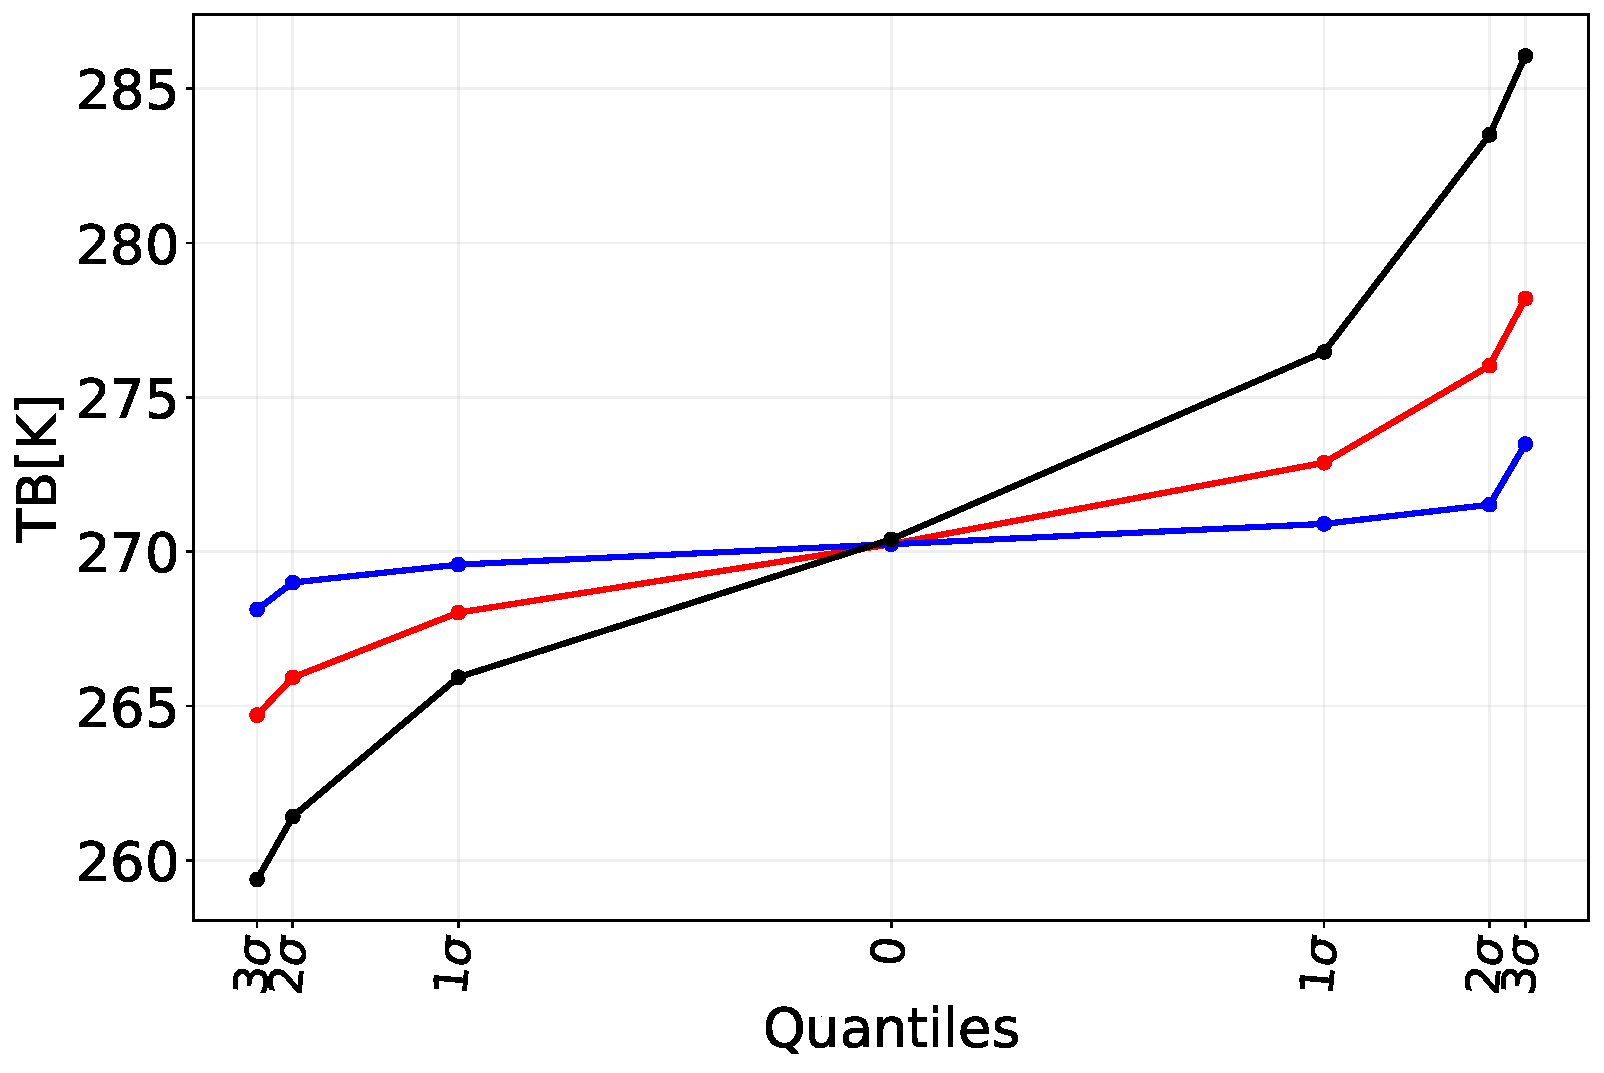
\includegraphics[height=45mm]{Figures/posterior_distribution_I1V.pdf} 
	\caption{An example showing the predicted quantiles of the conditional distribution of $\ynfcs$ }
	\label{fig:posterior_distribution_I1V}	
\end{figure}
QRNN predictions are posterior probability distribution of the NFCS values described over the selected quantiles. This is contrast with other conventional correction/filtering methods. In order to facilitate the interpretation of results, an example QRNN output is shown in Fig.~\ref{fig:posterior_distribution_I1V}. This examples illustrate the predicted quantiles for three different cases. For most analysis, usually a single point estimate is required. In Bayesian analysis, usually the posterior mean or posterior median are selected as point estimates. In this study, we assume the posterior median to be the best estimate for the predicted NFCS value ($\ynfcs$). To analyse the ability of QRNN in correctly predicting the point estimate, deviations of point estimates from the corresponding true value ($\yonfcs$) are evaluated using common performance indicators like bias, mean absolute error(MAE) and standard deviation (STD). The asymmetry of error distributions around their mean is also calculated through the measure of skewness. Fisher-Pearson coefficient of skewness is used to calculate the measure of skewness: 
\begin{equation}
g_1 = \frac{m_3}{m_2^{3/2}}, 
\end{equation}
where $m_2$ and $m_3$ are biased sample's second and third central moments.

For probabilistic predictions, accuracy of the point estimate is inadequate to gauge the complete performance. In a successful QRNN training, QRNN learns to predict not only an accurate point estimate but also correct underlying uncertainty. An ideal QRNN output should be sharp or in other words, concentrated in the vicinity of the point estimate. The predicted posterior distribution should also be well calibrated, that is, reflect the true probability distribution. A straightforward way to compare the two distribution is to plot the frequency of predictions and frequency of the true value in different prediction intervals. This is also commonly known as calibration plot. In a well-calibrated QRNN prediction, the calibration plot should follow the straight line y = x. Another way to assess how well the predicted posterior distribution reflects the observed errors is to compare predicted and observed errors. The predicted error is deviation of a random sample drawn from the posterior distribution to its median. In this study, we use both calibration plot and predicted errors to assess the correctness of predicted uncertainties.  

All evaluation results described in the study have been made on the testing data.


\section{Correcting cloud affected data in MWHS-2}
%
In this section, we introduce the QRNN based cloud  correction in the context of current operational sensors.  We use MWHS-2 to demonstrate the results. The choice is motivated by the fact that MWHS-2 has five complementary 183\,GHz channels as ATMS/MWS, along with additional 118\,GHz channel. In order to test the correction approach multiple QRNN experiments are performed and the results are compared for MWHS-2 channel 14. Later the methodology is expanded to other channels.  Further, the estimates of case-specific uncertainties obtained from QRNN are also evaluated.

\subsection{Experiments}
%
For MWHS-2, multiple experiments using both QRNN configurations are performed. The aim of the experiments is to delve into the sensitivity of the cloud correction to different input channels:

\begin{enumerate}
	
	\item In the first experiment, we examine the performance of QRNN cloud correction with MWHS-2 window channels: 89 and 150\,GHz. In ECMWF NWP system, the differences between the observations of these two window channels (Scattering Index) \citep{Lu2015FY3C} are used to identify the cloud affected data for ATMS, MHS and MWHS-2. To investigate the potential impact of window channels in QRNN based cloud correction, the configuration QRNN-single is applied to predict cloud free radiances. In this experiment, the training input includes all-sky brightness temperatures from target 183\,GHz channel, 89\,GHz and 150\,GHz. Both 89 and 150\,GHz are window channels so the land sea mask is also included as a training input. For example for channel 14, the training inputs are all-sky brightness temperatures from channels 14, 1, 10 and land/sea mask. This combination is referred as 89+150\,GHz in the text.
	
	\item In the second experiment, we explore if few of low peaking channels of 118\,GHz could have any potential advantage in cloud correction. To explore their impact, QRNN-single is trained with data from target 183\,GHz, 89\,GHz, 150\,GHz, 118.75$\pm$1.1\,GHz (channel 6), 118.75$\pm$2.5\,GHz (channel 7) and land/sea mask. This combination is denoted as 89+150+118\,GHz
	
	\item The third experiment is designed to assess the exclusive impact of 150\,GHz in cloud correction. In this experiment, QRNN-single is trained with brightness temperatures from 150\,GHz along with the target channel and land/sea mask. 
	
	\item The fourth experiment is based on the configuration QRNN-all. In this experiment, we use 89 and 150\,GHz channels along with all 183\,GHz channels to train QRNN. This experiment is motivated by the fact that in all-sky conditions, brightness temperatures between outer and inner humidity channels can be used as a criterion for cloud filtering\cite{buehler:aclou:07}. With QRNN-all, we investigate if additional humidity channels in the training process can improve the performance by providing auxiliary information. It should be noted that though the training inputs are same for each 183\,GHz channel, the output is the target 183\,GHz channel; thus each channel still needs to be trained separately. Land/sea mask is also included in the training. This combination is denoted as 89+150+183\,GHz
\end{enumerate}

\subsection{Prediction accuracy}

\subsubsection{QRNN-single applied to MWHS-2 channel 14} 
\begin{figure}[t]
	\centering
	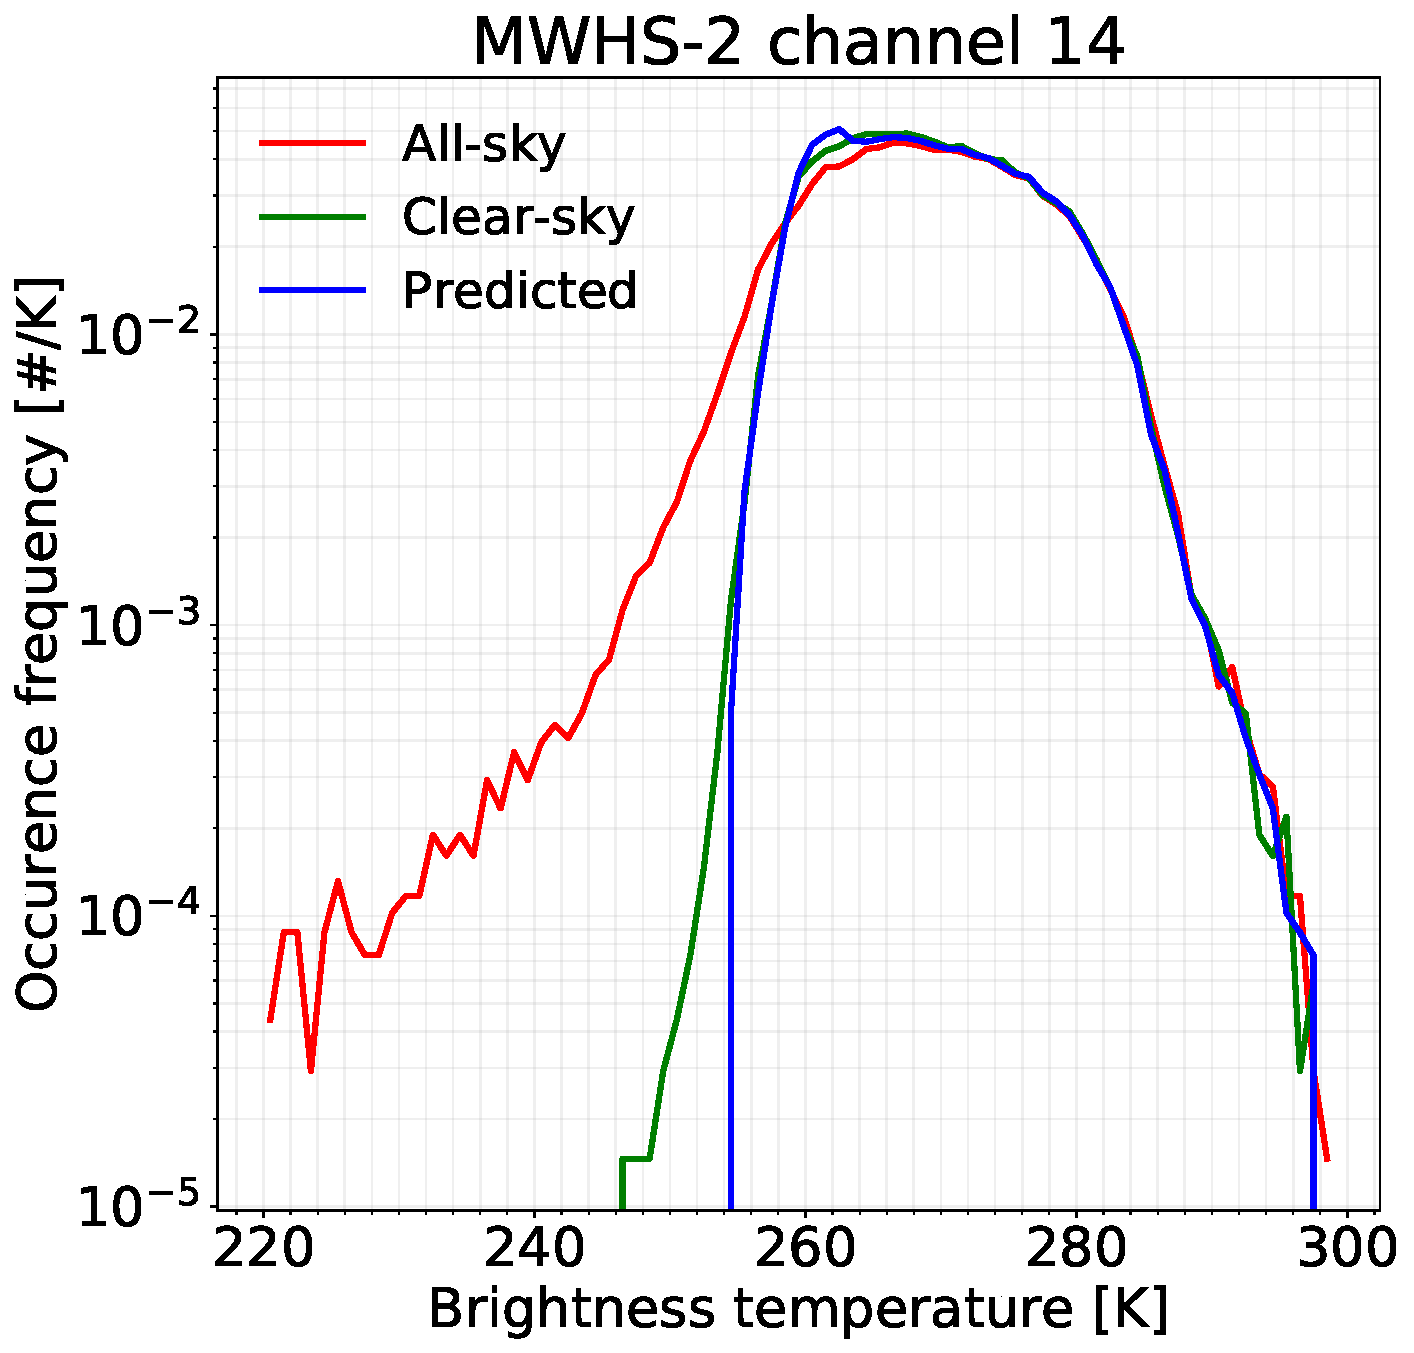
\includegraphics[height=55mm]{Figures/QRNN_output_mwhs.pdf} 
	\caption{Distributions of point estimate $\ynfcs$ obtained from QRNN-single 89+150\,GHz for MWHS-2 channel 14. The corresponding distribution for all-sky and clear-sky simulations are also shown.}
	\label{fig:distribution_predicted_mwhs14}	
\end{figure}
\begin{table*}[t]
	\caption{Error statistics for deviations of MWHS-2 NFSC predictions to simulations. Results are for different QRNN experiments for MWHS-2 channel 14. With configuration QRNN-single, the results are from combinations 89+150\,GHz, 89+150+118\,GHz and 150\,GHz. While with QRNN-all, only combination 89+150+183\,GHz is shown. The statistics for uncorrected all-sky simulations and NFCS simulations are also provided. The label ``All'' refers to entire predicted dataset, while Filtered(5\,K) denotes the subset where predictions with correction greater than 5\,K are omitted. The fraction of rejected cases is given in parentheses. }
	\label{tab:error_statistics_mwhs_14}
	\begin{tabular}{lrr|rr|rr|rr|rr}
		\tophline
		&\multicolumn{2}{c|}{Simulations}& \multicolumn{6}{c|}{QRNN-single} & \multicolumn{2}{c}{QRNN-all}\\
		\cline{2-11}
		%		\hline
		&   Clear-sky &   All-sky &  \multicolumn{2}{c|}{89+150\,GHz} & \multicolumn{2}{c|}{89+150+118\,GHz} & \multicolumn{2}{c|}{150\,GHz} & \multicolumn{2}{c}{89+150+183\,GHz}\\
		&			   &			& All & Filtered(5K) & All & Filtered(5K) & All & Filtered(5K)  & All & Filtered(5K)\\
		\middlehline
		bias     &  0.00 &  -0.84 & -0.09 & -0.08(3.3\%) & -0.04 & -0.03(3.4\%) & -0.09 & -0.09(3.2\%) & -0.09(3.3\%) & -0.08(3.3\%)  \\
		mae      &  0.80 &   1.45 &  0.88 &  0.86 &  0.89 &  0.87 &  0.89 &  0.87 &  0.62 &  0.59\\
		std      &  1.00 &   3.90 &  1.19 &  1.14 &  1.19 &  1.15 &  1.21 &  1.16 &  0.90 &  0.83\\
		skewness & -0.00 & -14.34 & -1.11 & -0.93 & -1.00 & -0.84 & -0.88 & -0.98 & -1.58 & -1.62\\
		\bottomhline
	\end{tabular}
\end{table*}
Fig.~\ref{fig:distribution_predicted_mwhs14} shows the distribution of QRNN predictions obtained from QRNN. QRNN predictions are able to remove the extended mass concentration to the left is due hydrometeor impact, and overall a good match with the NFCS simulations is observed. QRNN is unable to predict the lowest clear-sky brightness temperatures, but cases with brightness temperatures around 260\,K occur frequently.  Table~\ref{tab:error_statistics_mwhs_14} shows the error statistics for the predictions shown in Fig.~\ref{fig:distribution_predicted_mwhs14}. In the uncorrected data, cloud impact causes a large negative skewness(-14.34) in the error distribution and the corresponding bias is -0.84\,K. Training QRNN with 89 and 150\,GHz removes a part of the cloud impact and reduces the bias to -0.09\,K, and the skewness is -1.11. The MAE and STD are also reduced after correction, but are higher than noise. Including 118\,GHz in the training, gives comparable results as 89+150\,GHz. With 118\,GHz, the error distributions have lower bias and are more symmetric, but the MAE and STD remain unaltered. This indicates that the information from 118\,GHz channels can be beneficial in predicting few cases correctly, but the overall consequence is not exceptionally different from 89+150\,GHz. Similar is the case with using only 150\,GHz. In the latter, predictions have the most symmetric  error distributions, but the highest spread. 

Further we investigated that if filtering the predictions with large residual cloud impact could help in improving the prediction accuracy. For filtering such cases, we assume that predictions with cloud correction greater than 5\,K are cases associated with large deviations. In all three experiments, removing the cases with correction greater than 5\,K removes around 3\% of the data, but only a marginal positive impact on the accuracy is observed. With 5\,K thresold, though the cases with high errors are removed, the negative skewness conveys that some cases with low cloud impact are not completely corrected. Choosing a lower threshold can help in removing more partially corrected cases but at the cost of rejecting clear-sky cases. Since QRNN gives out NFCS values, choosing an unusually low correction threshold can also classify noisy clear-sky cases as cloudy. For example, for 89+150\,GHz, a threshold of 1.5\,K rejects almost 10\% of data, but the negative skewness is still not completely removed. 

In spite of the fact that QRNN only provides a partial cloud correction, the results are better to what scattering index (SI) based approach would give. SI uses the differences of brightness temperatures between 89 and 150\,GHz to identify cloud affected data \citep{geer2015scatteringindex}. With 5\,K SI threshold, almost 30\% of the data is rejected and the error distributions have bias, mae and standard deviation as -0.23\,K 0.92\,K and 1.40\,K respectively (Table~\ref{tab:SI_statistics}). 

The three experiments were also performed for other four 183\,GHz channels, and a similar performance was obtained (Table not shown). The positive effect of 118\,GHz was slightly higher for MWHS-2 channel 15, but for others, no notable effect was observed. The results from combination 89+150\,GHz for these channels are provided in Sect.~\ref{sec:mwhs_others} 

\subsubsection{Comparison of QRNN-all and QRNN-single}
%
%f
\begin{figure}[t]
	\centering
	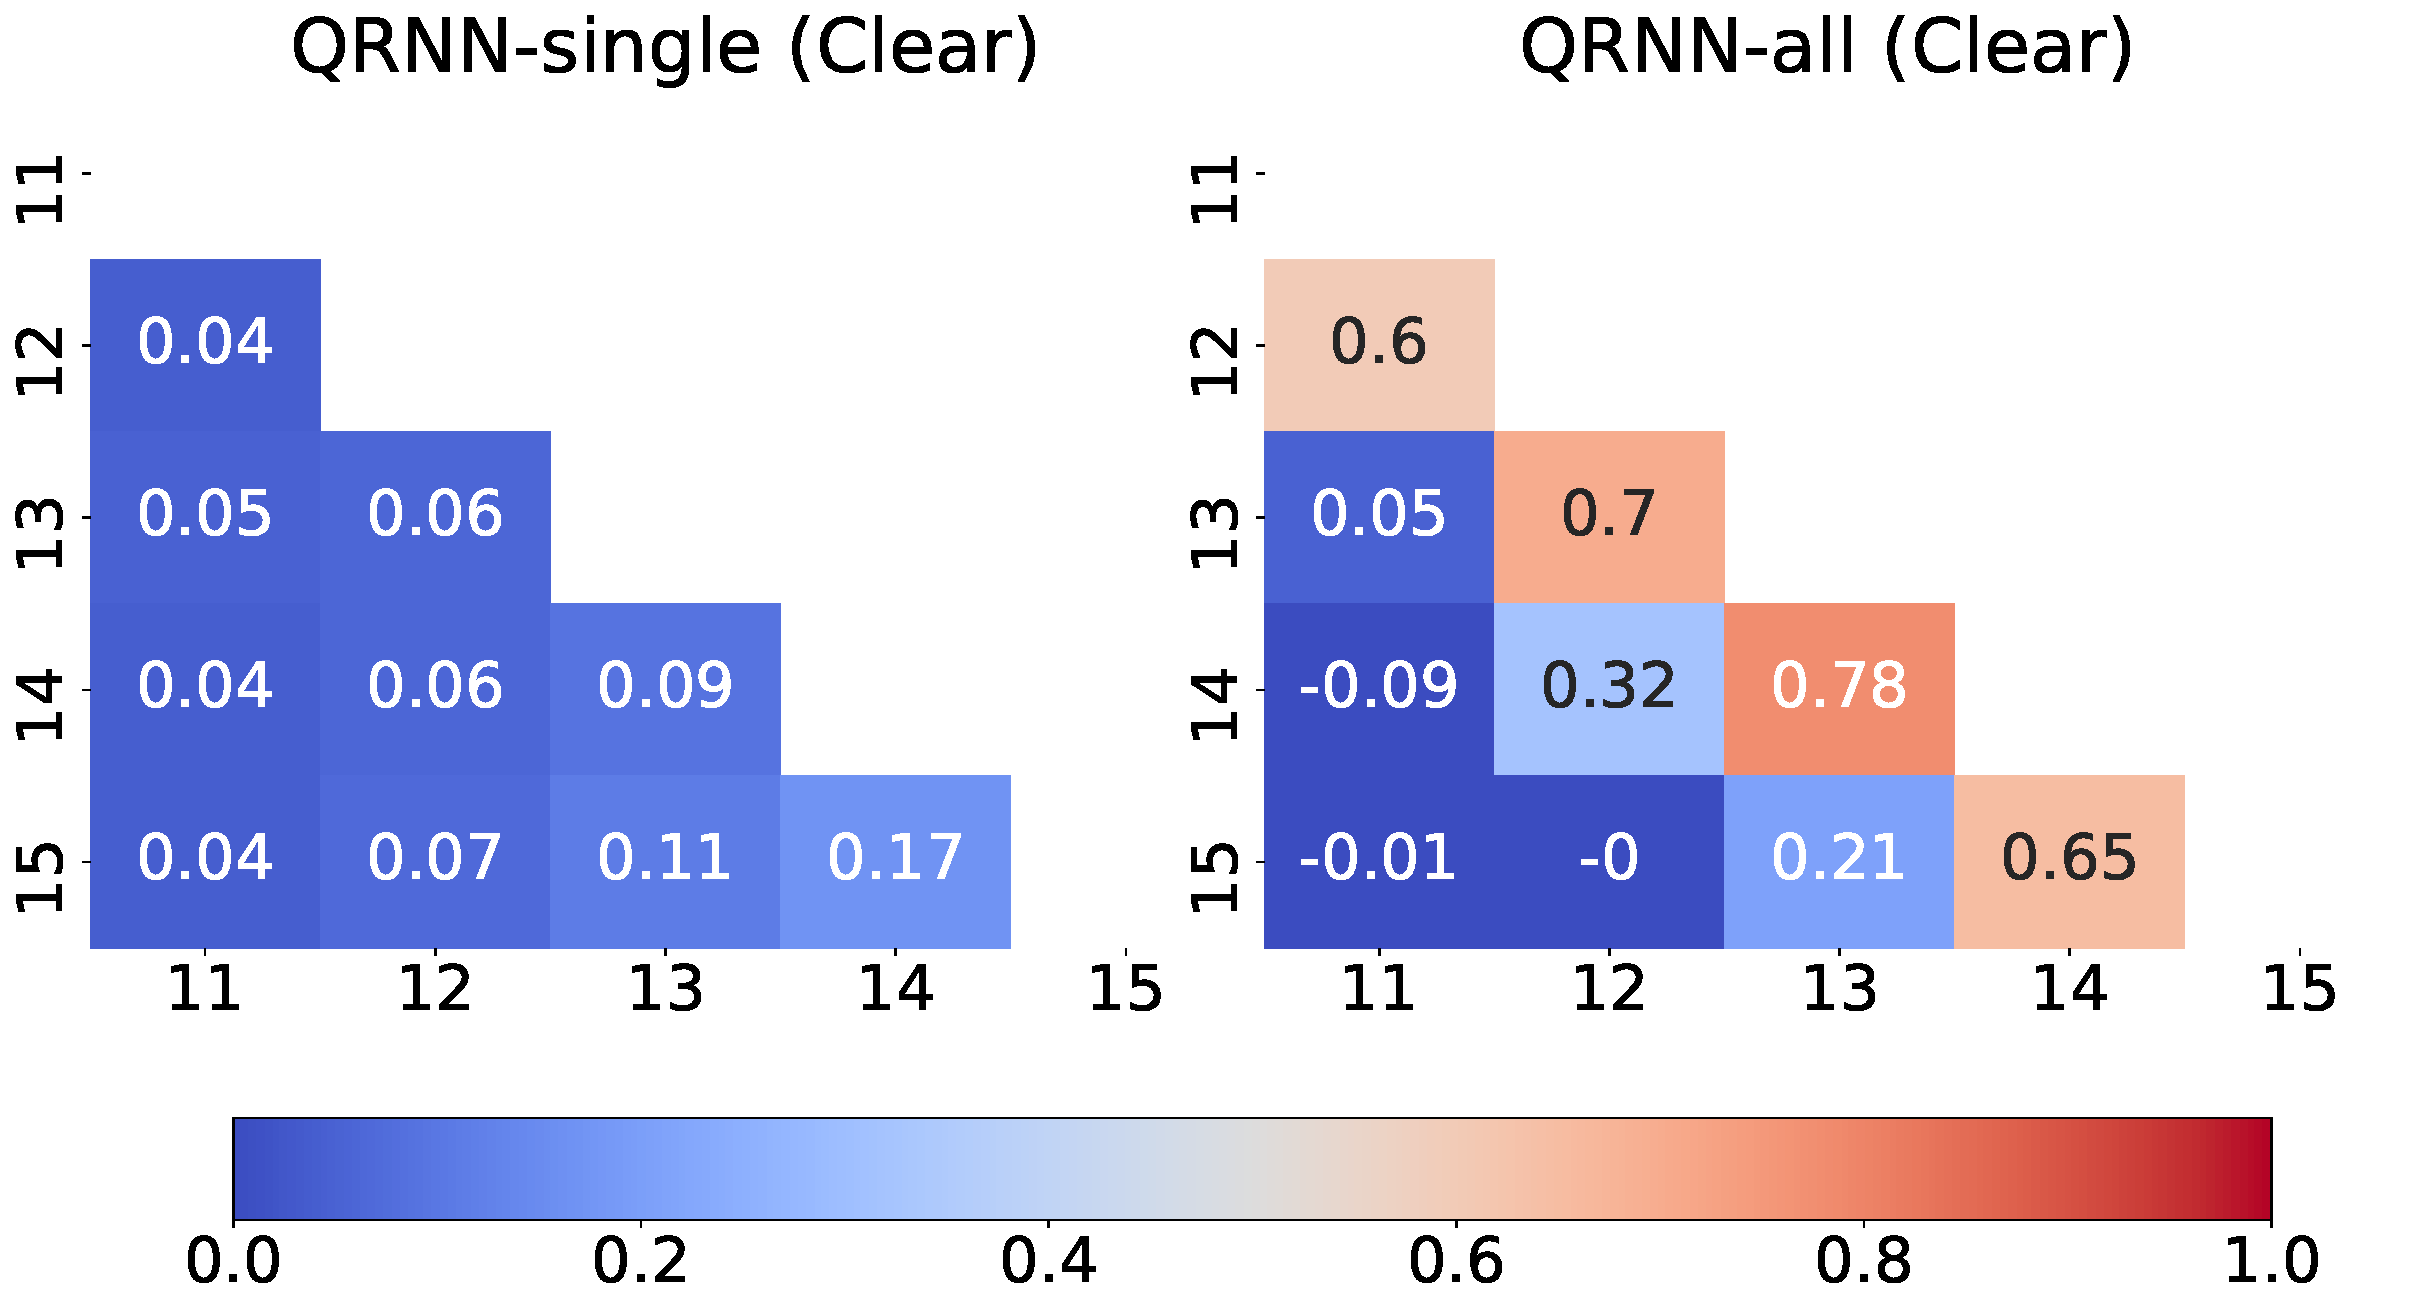
\includegraphics[height=45mm]{Figures/correlation.pdf} 
	\caption{ The triangular error correlation matrix obtained from QRNN-single and QRNN-all for MWHS-2. The label ``Clear'' represents cases with cloud impact less than 2\,K.}
	\label{fig:correlations_mwhs}	
\end{figure}
To assess the differences between the capabilities of QRNN-all against QRNN-single, we  compare the error statistics obtained for 89+150\,GHz and 89+150+183\,GHz for channel 14. The last column of Table~\ref{tab:error_statistics_mwhs_14} displays the error statistics for the experiment QRNN-all. In comparison to QRNN-single, we obtain marginally lower error bias with QRNN-all, and the MAE and standard deviation reduce by almost 30\% and 25\% respectively. However the negative tail becomes more prominent. The low standard deviation, but strong negative tail indicates that the narrow spread is a consequence of correction of noise in clear-sky cases. Since a majority of the cases are clear-sky, their impact dominates the whole statistics. In order to quantify the positive effect of QRNN-all on cases with high and low cloud impact, a separate analysis of the high and low cloud impact cases is made. In both cases, QRNN-all has slightly better accuracy than QRNN-single, suggesting that concurrent use of all 183\,GHz channels can provide additional information on cloud structures to QRNN. 

Even though QRNN-all gives slightly better prediction accuracy, its inherent construction makes it crucial to examine the correlation between observed errors. Fig~\ref{fig:correlations_mwhs} illustrates the correlation matrix for both QRNN-all and QRNN-single. For clear cases, the observed errors (noise) in QRNN-single are uncorrelated between the five channels. However QRNN-all gives out highly correlated errors. The correlations are highest between adjacent channels, and drop out as the spacing between the channels increases. For cloudy cases, the observed errors obtained from QRNN-single are slightly correlated, but with QRNN-all a very strong correlation is observed(not shown). The residual cloud amount for different channels depends upon each other in a systematic way, but since QRNN-single does not have access to this information, only slightly higher correlations are observed. On the other hand, with QRNN-all, when all 183\,GHz channels are used simultaneously the predictions learn positively from the common information and also introduces high correlations between overlapping channels. Correlated errors can be undesirable for DA systems, so the configuration QRNN-all is avoided for further development.


\subsubsection{QRNN-single applied to channel 11, 12, 13 and 15}
\label{sec:mwhs_others}
\begin{table*}[t]
	\caption{ Error statisics for MWHS-2 channels 11, 12, 13 and 15 from QRNN-single experiment 89+150\,GHz. The labels ``All'' and ``Filtered(5\,K)' are as described in Table~\ref{tab:error_statistics_mwhs_14}.}
	\label{tab:error_statistics_mwhs_others}
	\begin{tabular}{lrrr|rr}
		\tophline
		&&\multicolumn{2}{c|}{Simulations}& \multicolumn{2}{c}{QRNN-single} \\
		\cline{2-6}
		%		\hline
		& &  Clear-sky &   All-sky &  \multicolumn{2}{c}{89+150\,GHz}  \\
		&	&		   &			& All & Filtered(5K)\\
		\middlehline
		Channel 11  &   bias     & 0.00 &  -0.16 & -0.03 & -0.03(0.2\%)  \\
				    &	mae      & 0.80 &   0.89 &  0.79 &  0.79  \\
					&	std      & 1.00 &   1.71 &  1.03 &  1.01  \\
					&	skewness & 0.01 & -20.18 & -0.68 & -0.45  \\
		\middlehline
		Channel 12  & bias     & -0.00 &  -0.28 & -0.05 & -0.05(0.6\%)  \\
					& mae      &  0.80 &   0.98 &  0.81 &  0.80  \\
					& std      &  1.00 &   2.26 &  1.07 &  1.05  \\
					& skewness &  0.00 & -20.72 & -0.91 & -0.70  \\
		\middlehline
		Channel 13  & bias     & -0.00 &  -0.52 & -0.08 & -0.07(1.6\%)  \\
					& mae      &  0.80 &   1.17 &  0.84 &  0.83  \\
					& std      &  1.00 &   3.04 &  1.13 &  1.10  \\
					& skewness &  0.02 & -17.85 & -1.14 & -0.98 \\		
		\middlehline
		Channel 15  & bias     & -0.00 &  -1.28 & -0.07 & -0.06(5.6\%)  \\
					& mae      &  0.80 &   1.87 &  0.97 &  0.92 \\
					& std      &  1.00 &   5.08 &  1.35 &  1.25 \\
					& skewness & -0.00 & -11.15 & -0.60 & -0.83  \\ 
		\bottomhline
	\end{tabular}
\end{table*}
\begin{table}[t]
	\caption{Error statistics obtained after filtering MWHS-2 humidity observations according to scattering index.  }
	\label{tab:SI_statistics}
	\begin{tabular}{lrrrrr}
		\tophline
		& Ch. 11 & Ch. 12 & Ch. 13 & Ch. 14 & Ch. 15\\
			\cline{2-6}
		bias     & -0.05&  -0.07 & -0.14 & -0.23 &  -0.34\\
		mae      & 0.81 &   0.82 &  0.85 &  0.92 &  1.03\\
		std      & 1.02 &   1.04 &  1.10 &  1.25 &  1.53\\
		\bottomhline
	\end{tabular}
\end{table}

In this section, we extend QRNN-single to predict NFCS values for MWHS-2 channels 11, 12, 13, and 15. The experiment QRNN-single with combination 89+150\,GHz is used and the results are displayed in  Table~\ref{tab:error_statistics_mwhs_others}.

For channel 11, the error bias after correction is only -0.03\,K in comparison to 0.16\,K before correction. The strong negative tail also diminishes after correction, but a non-zero negative skewness indicates presence of cases with cloud impact in the corrected dataset. Filtering the cases with high cloud impact has only a marginally positive impact. A similar performance is evident for channel 12. Correction reduces the bias to -0.05\,K and the MAE is approximately 17\% lower for the entire test dataset. However the effect of partially corrected cases is evident in the negative skewness. There is again only a partial correction evident for channels 13 and 15. The bias values are quite low indicating that QRNN is successful in removing a large fraction of the cloud impact, but relatively high skewness is a consequence of cases with low cloud impact which end up with inadequate correction.  

A comparison with SI based filtering is also made (Table~\ref{tab:SI_statistics}). For channels 11 and 12 the performance of QRNN is comparable to scattering index, albeit 30\% of the observations are rejected in the latter. For channels 13 and 15, the error statistics obtained with SI are slightly worse.   


\subsection{Prediction uncertainty}

\begin{figure}[t]
	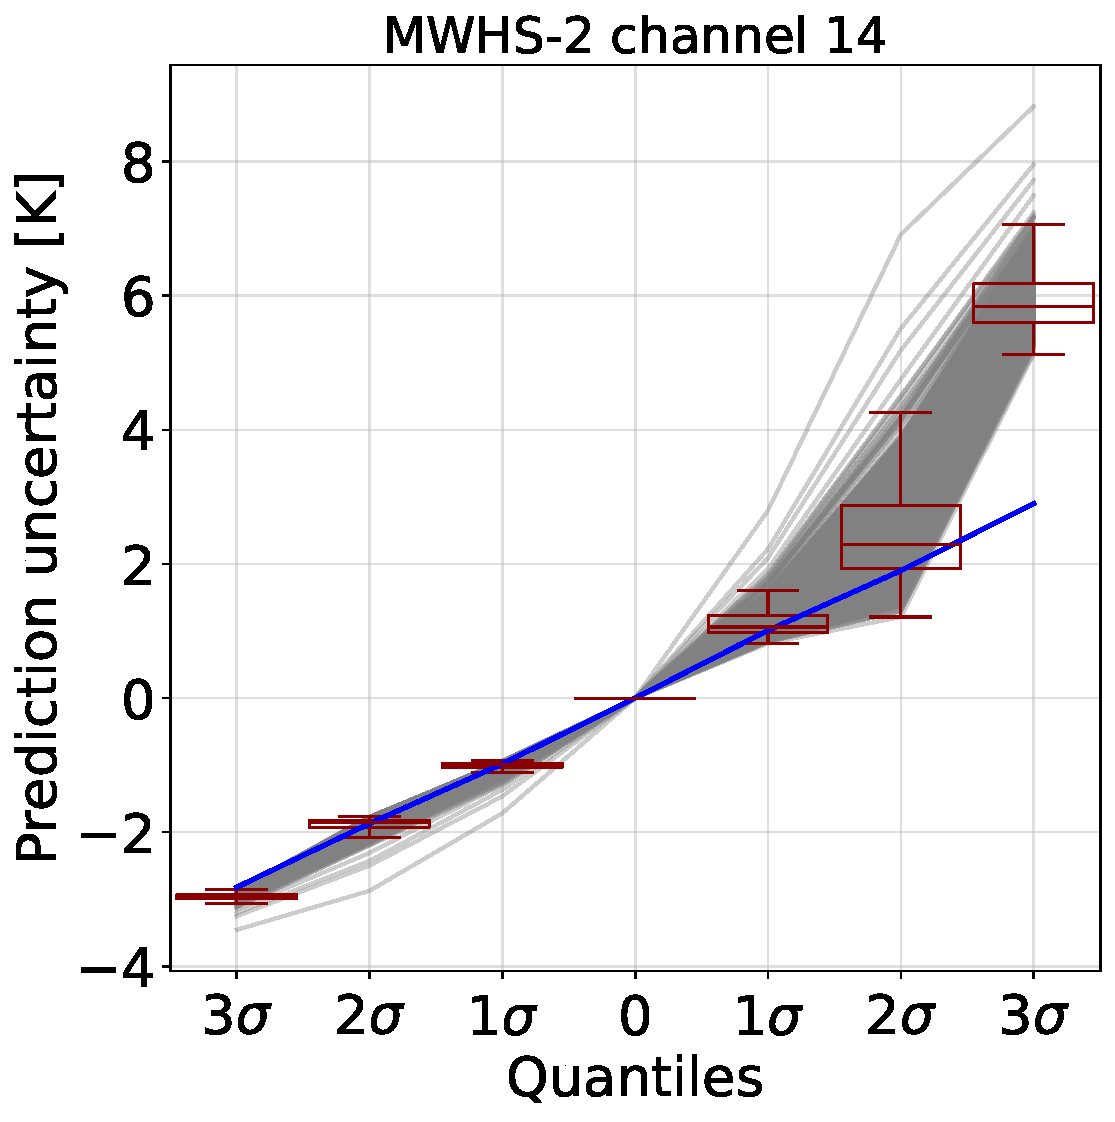
\includegraphics[width = 70mm]{Figures/prediction_uncertainty_MWHS_14.pdf}	
	\caption{The prediction uncertainty for MWHS-2 channel 14 (QRNN-single) with respect to quantiles for randomly selected 1500 cases. The quantiles have been plotted at equidistant points. The red line represents a hypothetical Gaussian distribution of $270\pm1.0$\,K.}
	\label{fig:prediction_uncertainty_mwhs}	
\end{figure}
\begin{figure}[t]
	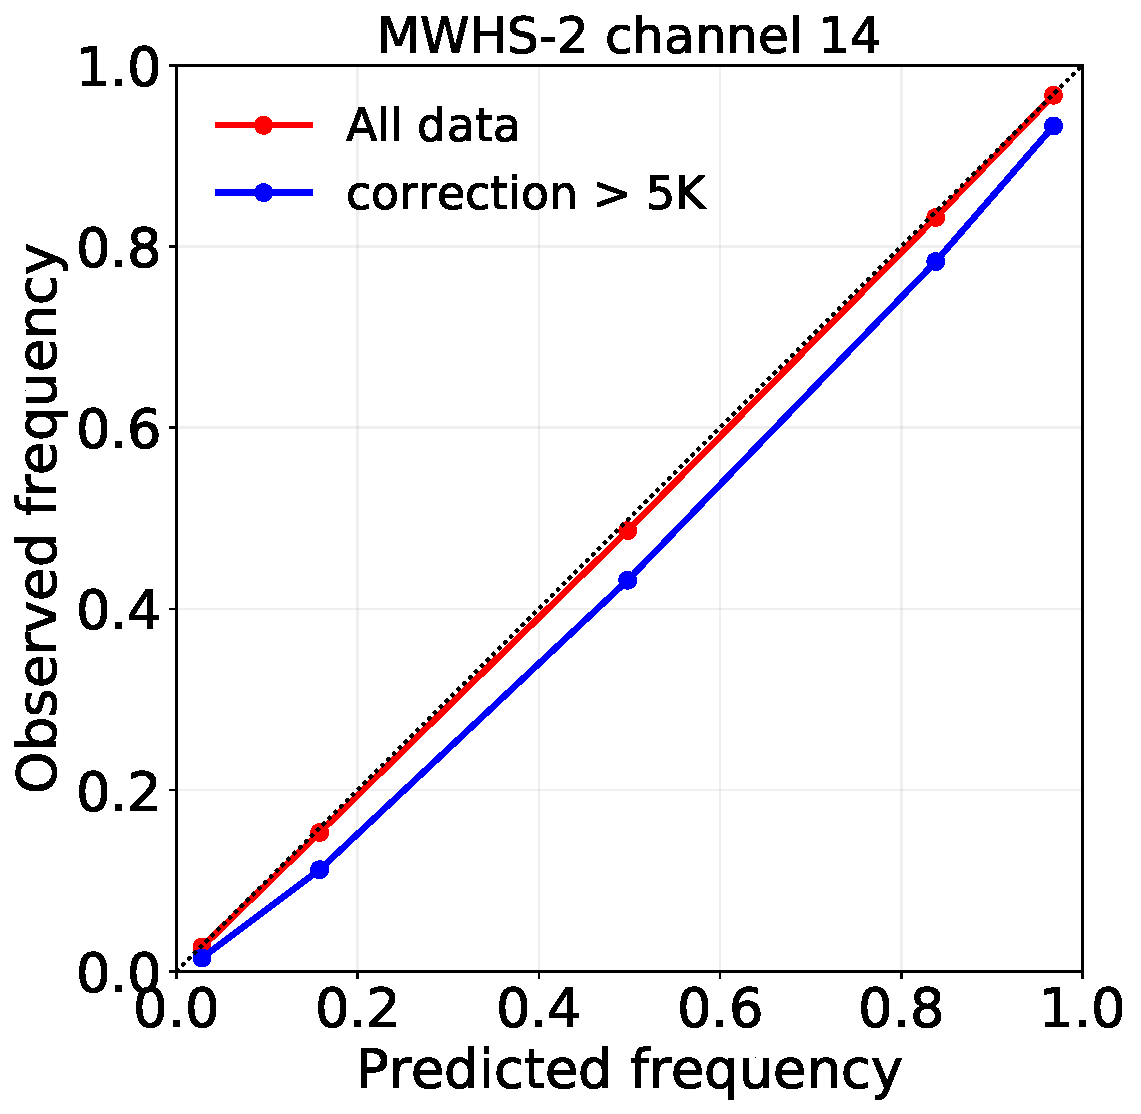
\includegraphics[height = 70mm]{Figures/calibration_QRNN_MWHS_14.pdf}	
	\caption{Calibration of the prediction intervals obtained from QRNN-single for MWHS-2 channel 14. }
	\label{fig:calibration_mwhs}	
\end{figure}
\begin{figure}[t]
	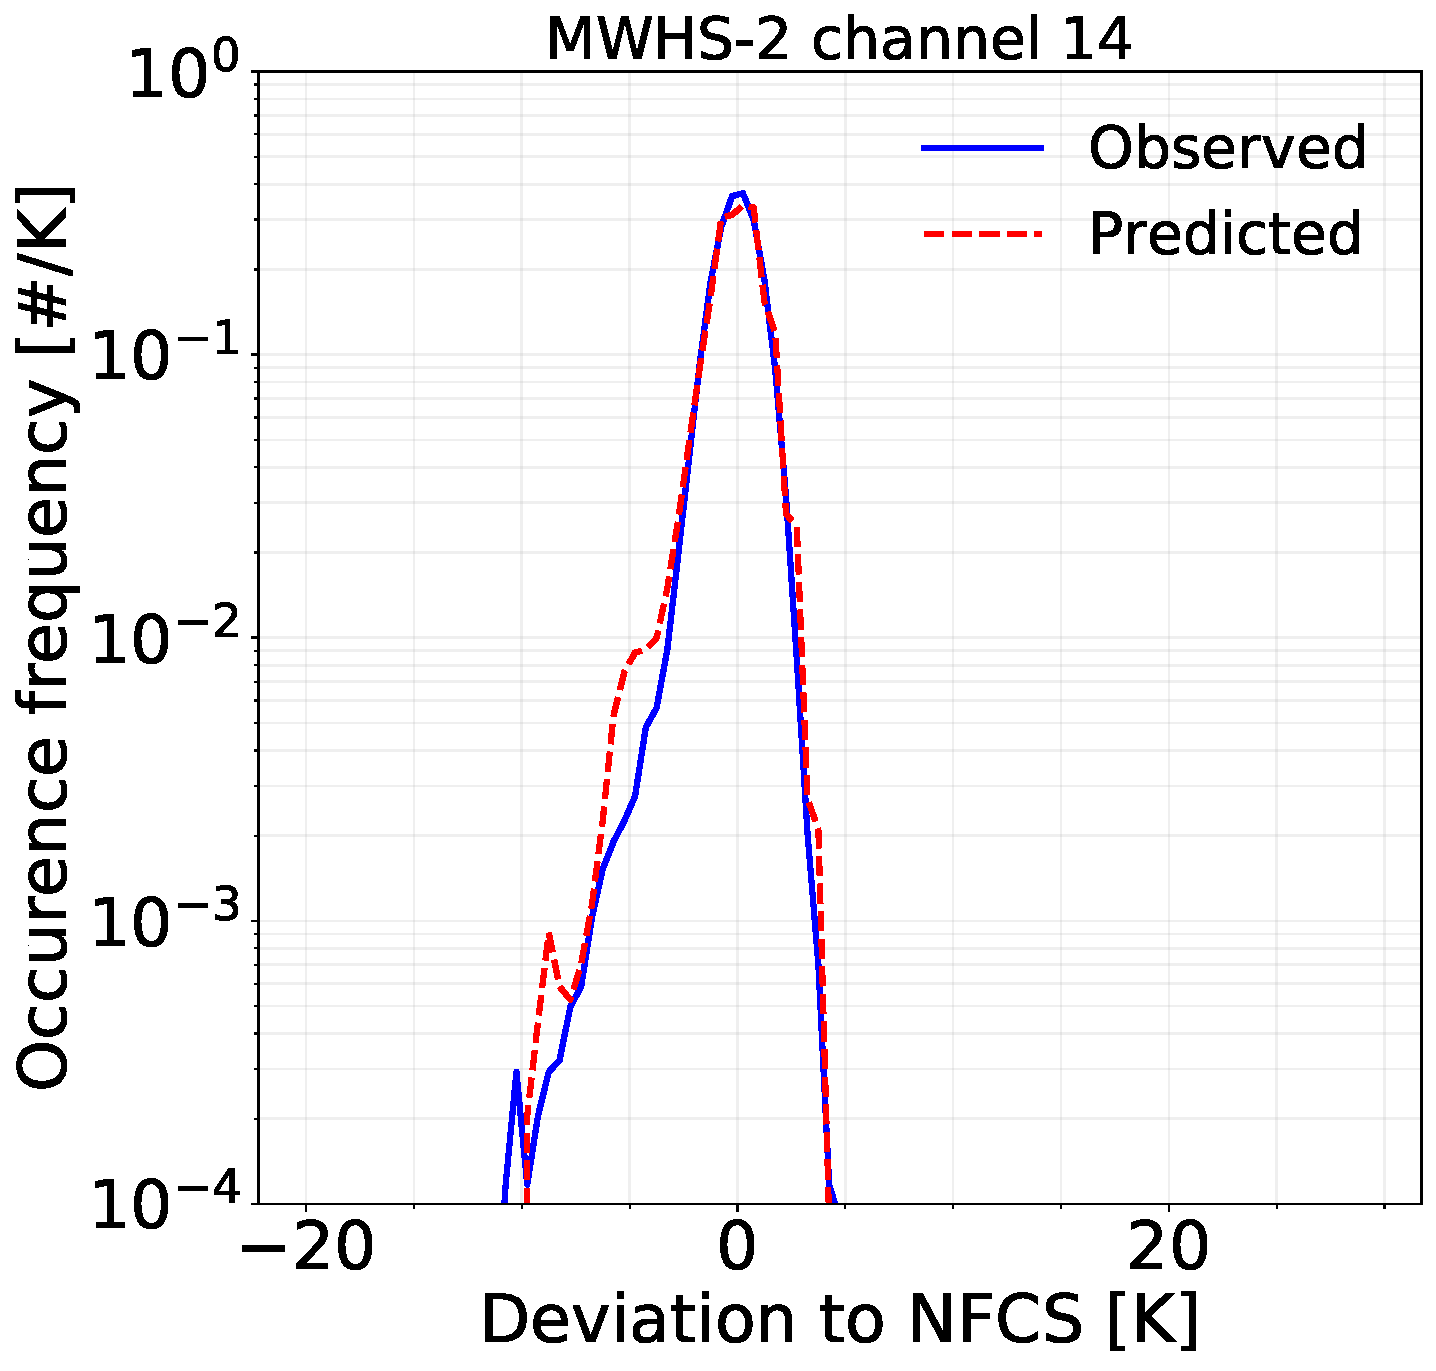
\includegraphics[width=70mm]{Figures/deviation_posterior_mwhs_samples_14.pdf}	
	\caption{The distribution of predicted errors and observed errors for MWHS-2 channel 14 as obtained from QRNN-single for the test dataset. The predicted errors are estimated as deviation of random samples from posteriori distribution to corresponding median values.}
	\label{fig:predicted_errors_mwhs}	
\end{figure}

The quantiles given out by QRNN can be used to construct the probability distribution of the predictions in contrast to other correction approaches which give out only point estimates.  

An example of the uncertainties given out by QRNN is shown in Fig~\ref{fig:prediction_uncertainty_mwhs}. The predictions over quantiles $-3\sigma$, $-2\sigma$ and $-1\sigma$ are quite sharp and lie close to the median value. The spread over different cases is also quite narrow, with only few cases with high error. In contrast, the spread of predictions over quantiles $1\sigma$, $2\sigma$ and $3\sigma$ is wider. 

The calibration of the prediction intervals on the testing dataset is displayed in Fig~\ref{fig:calibration_mwhs}. For the entire testing dataset, the predictions follow the y=x line, i.e. they are perfectly calibrated with the priori distribution. However for all cases with correction greater than 5\,K, the distribution is poorly calibrated. In this case, the calibration curve lies below the y=x line indicating that the prediction intervals are too narrow.  However since such cases are few and filtering them out results in well calibrated QRNN predictions. 

Further we analysed if the  predicted errors obtained from QRNN are representative of observed errors. Fig~\ref{fig:predicted_errors_mwhs} illustrates the predicted and observed errors for MWHS-2 channel 14. The predicted errors are slightly overestimated for negative values, but overall the predicted errors from the QRNN posterior distribution have a good match with the observed errors. This is in agreement with the perfect calibration seen in Fig.~\ref{fig:calibration_mwhs}. It should be noted that the density plot is curtailed at $10^{-4}$. With a test dataset of 70\,000 samples, we cannot represent the far wings of the distribution accurately. The high errors which we try to estimate are rare, and can not be fully represented by QRNN. 

For other humidity channels, the predicted uncertainties followed similar behaviour and the not shown. 


\section{Correcting cloud affected data using sub-mm frequencies}
In this section, we demonstrate that sub-mm channels can be used to formulate the cloud correction of data measured around 183\,GHz. Results from different QRNN experiments with varying input conditions are described. The results are presented in context of different sensors. Furthermore, the case specific uncertainties predicted by QRNN are also discussed.

\subsection{Experiments}
%
Two QRNN experiments are performed to investigate the efficacy of sub-mm channels in cloud correction: 
\begin{enumerate}
	\item In the first experiment, we follow the QRNN-single configuration to for cloud correction at three ICI humidity channels. In this case, the training data is the target 183\,GHz channel and all available ICI sub-mm frequencies (325\,GHz, 448\,GHz and 664\,GHz). No other data are included in the training process. The experiment is also channel specific, thus each 183\,GHz channel is trained separately. For example, to predict NFCS values for channel I1V, the input training dataset includes noisy all-sky simulations from channels I1V, I5V, I6V, I7V, I8V, I9V, I10V, and I11V and the target is NFCS simulations for channel I1V.
	
	\item In the second experiment, we investigate the possibility of using only channels around 325\,GHz for cloud correction at 183\,GHz. This special case of utilising only 325\,GHz channel can be relevant for smaller satellite missions like AWS where higher sub-mm channels are not available. In this experiment, QRNN-single configuration is used and it is trained with all-sky simulations from all 325\,GHz frequencies from AWS and the target 183\,GHz channel. For example, for target AWS-32, the training inputs were AWS-32, AWS-41, AWS-42, AWS-43, AWS-44. QRNN was trained five times for each 183\,GHz channel as target. 	
\end{enumerate}	

\subsection{Prediction accuracy}
\subsubsection{ICI}
%
%f
\begin{figure*}[t]
	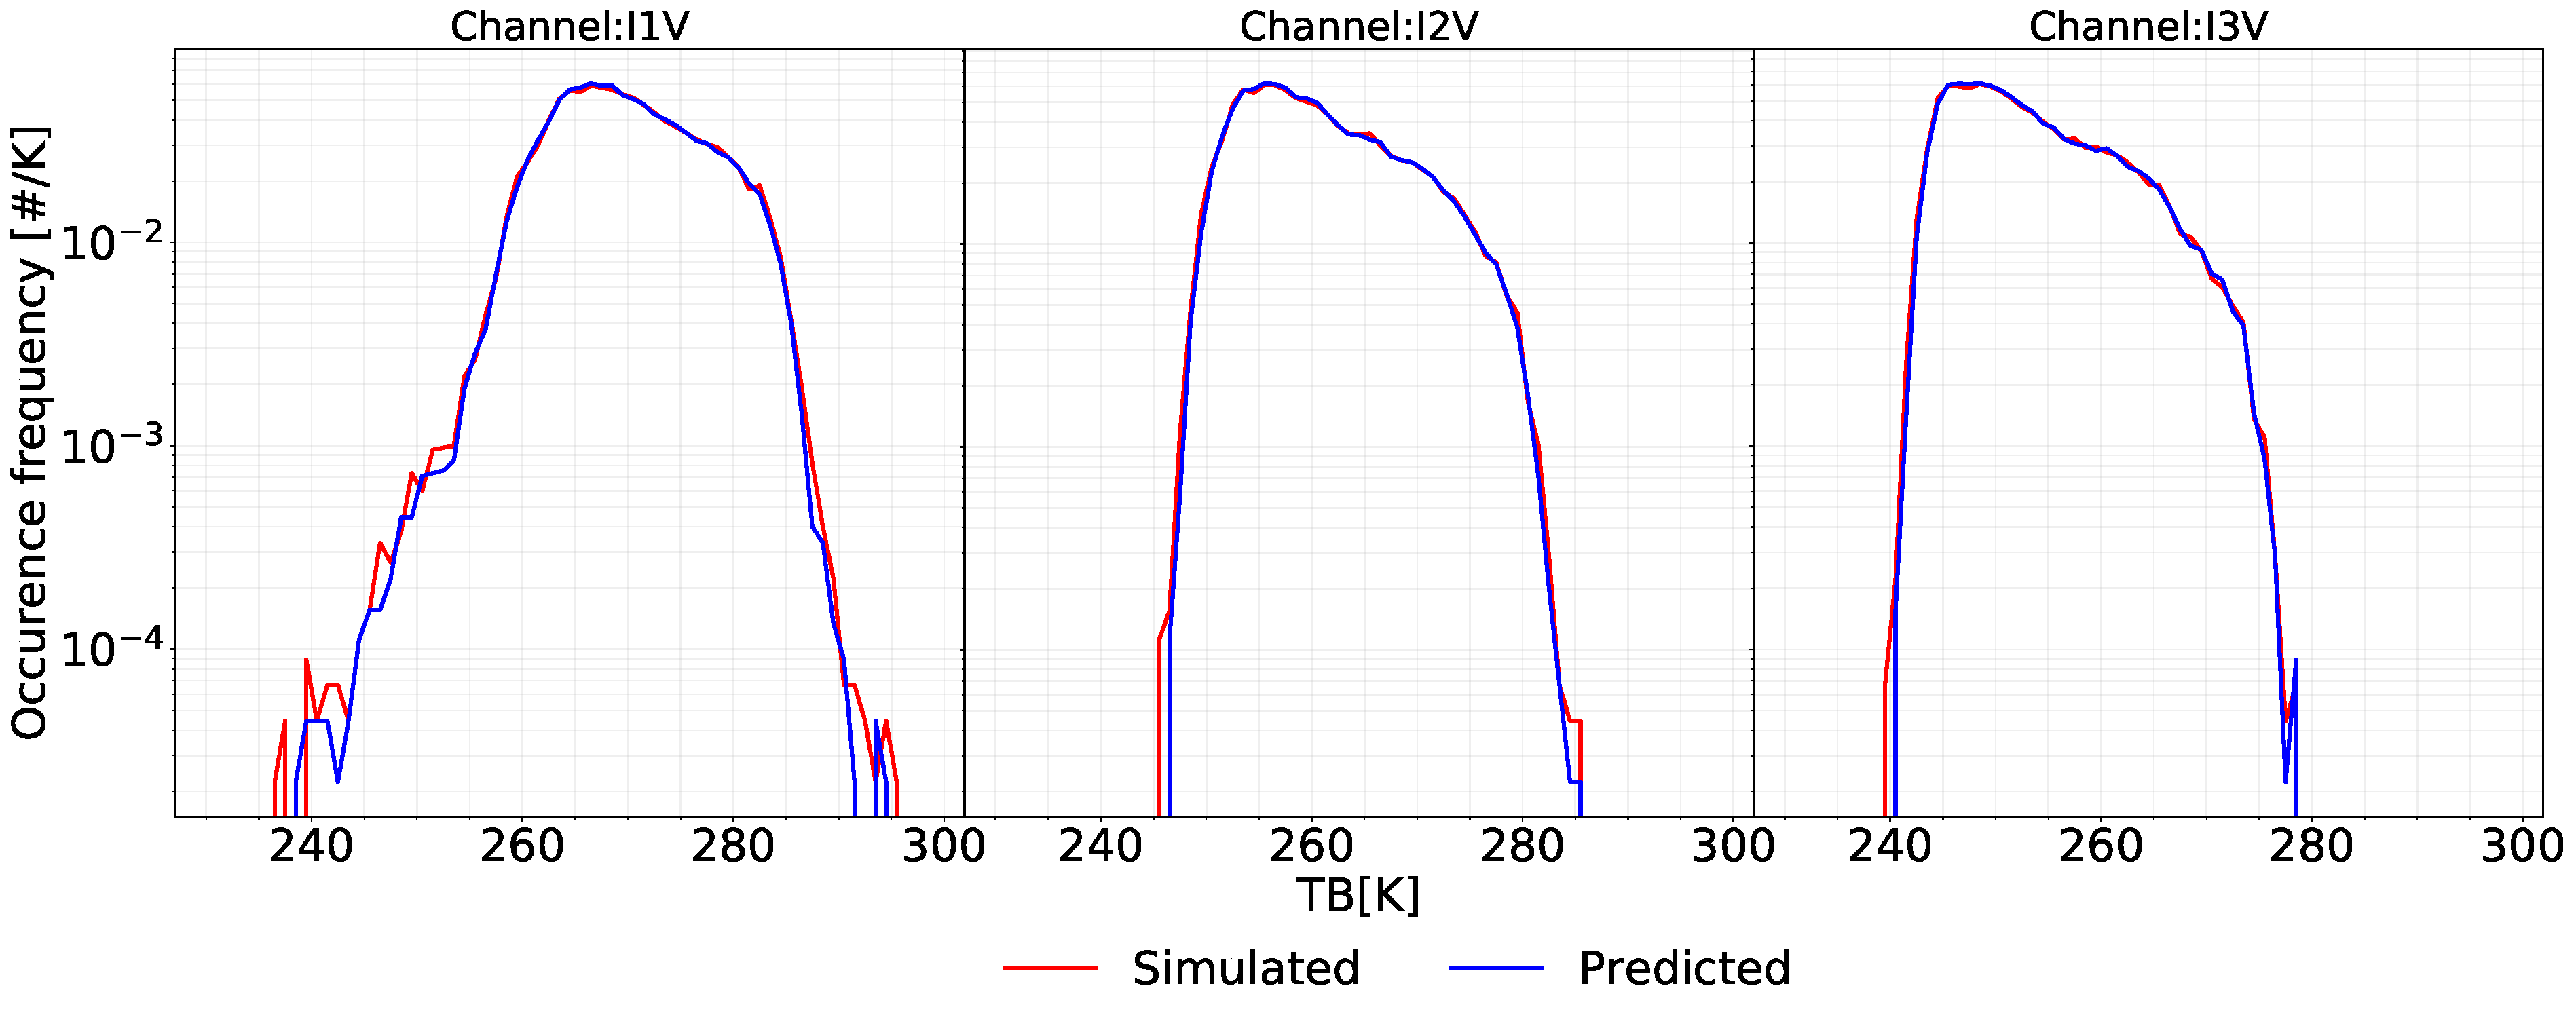
\includegraphics[width=\textwidth]{Figures/PDF_predictions_ICI.pdf} 
	\caption{Distributions of point estimate NFCS from QRNN-single for channels I1V, I2V and I3V. The corresponding distributions for NFCS simulations are also shown.}
	\label{fig:PDF_predictions}	
\end{figure*}
\begin{figure*}[t ]
	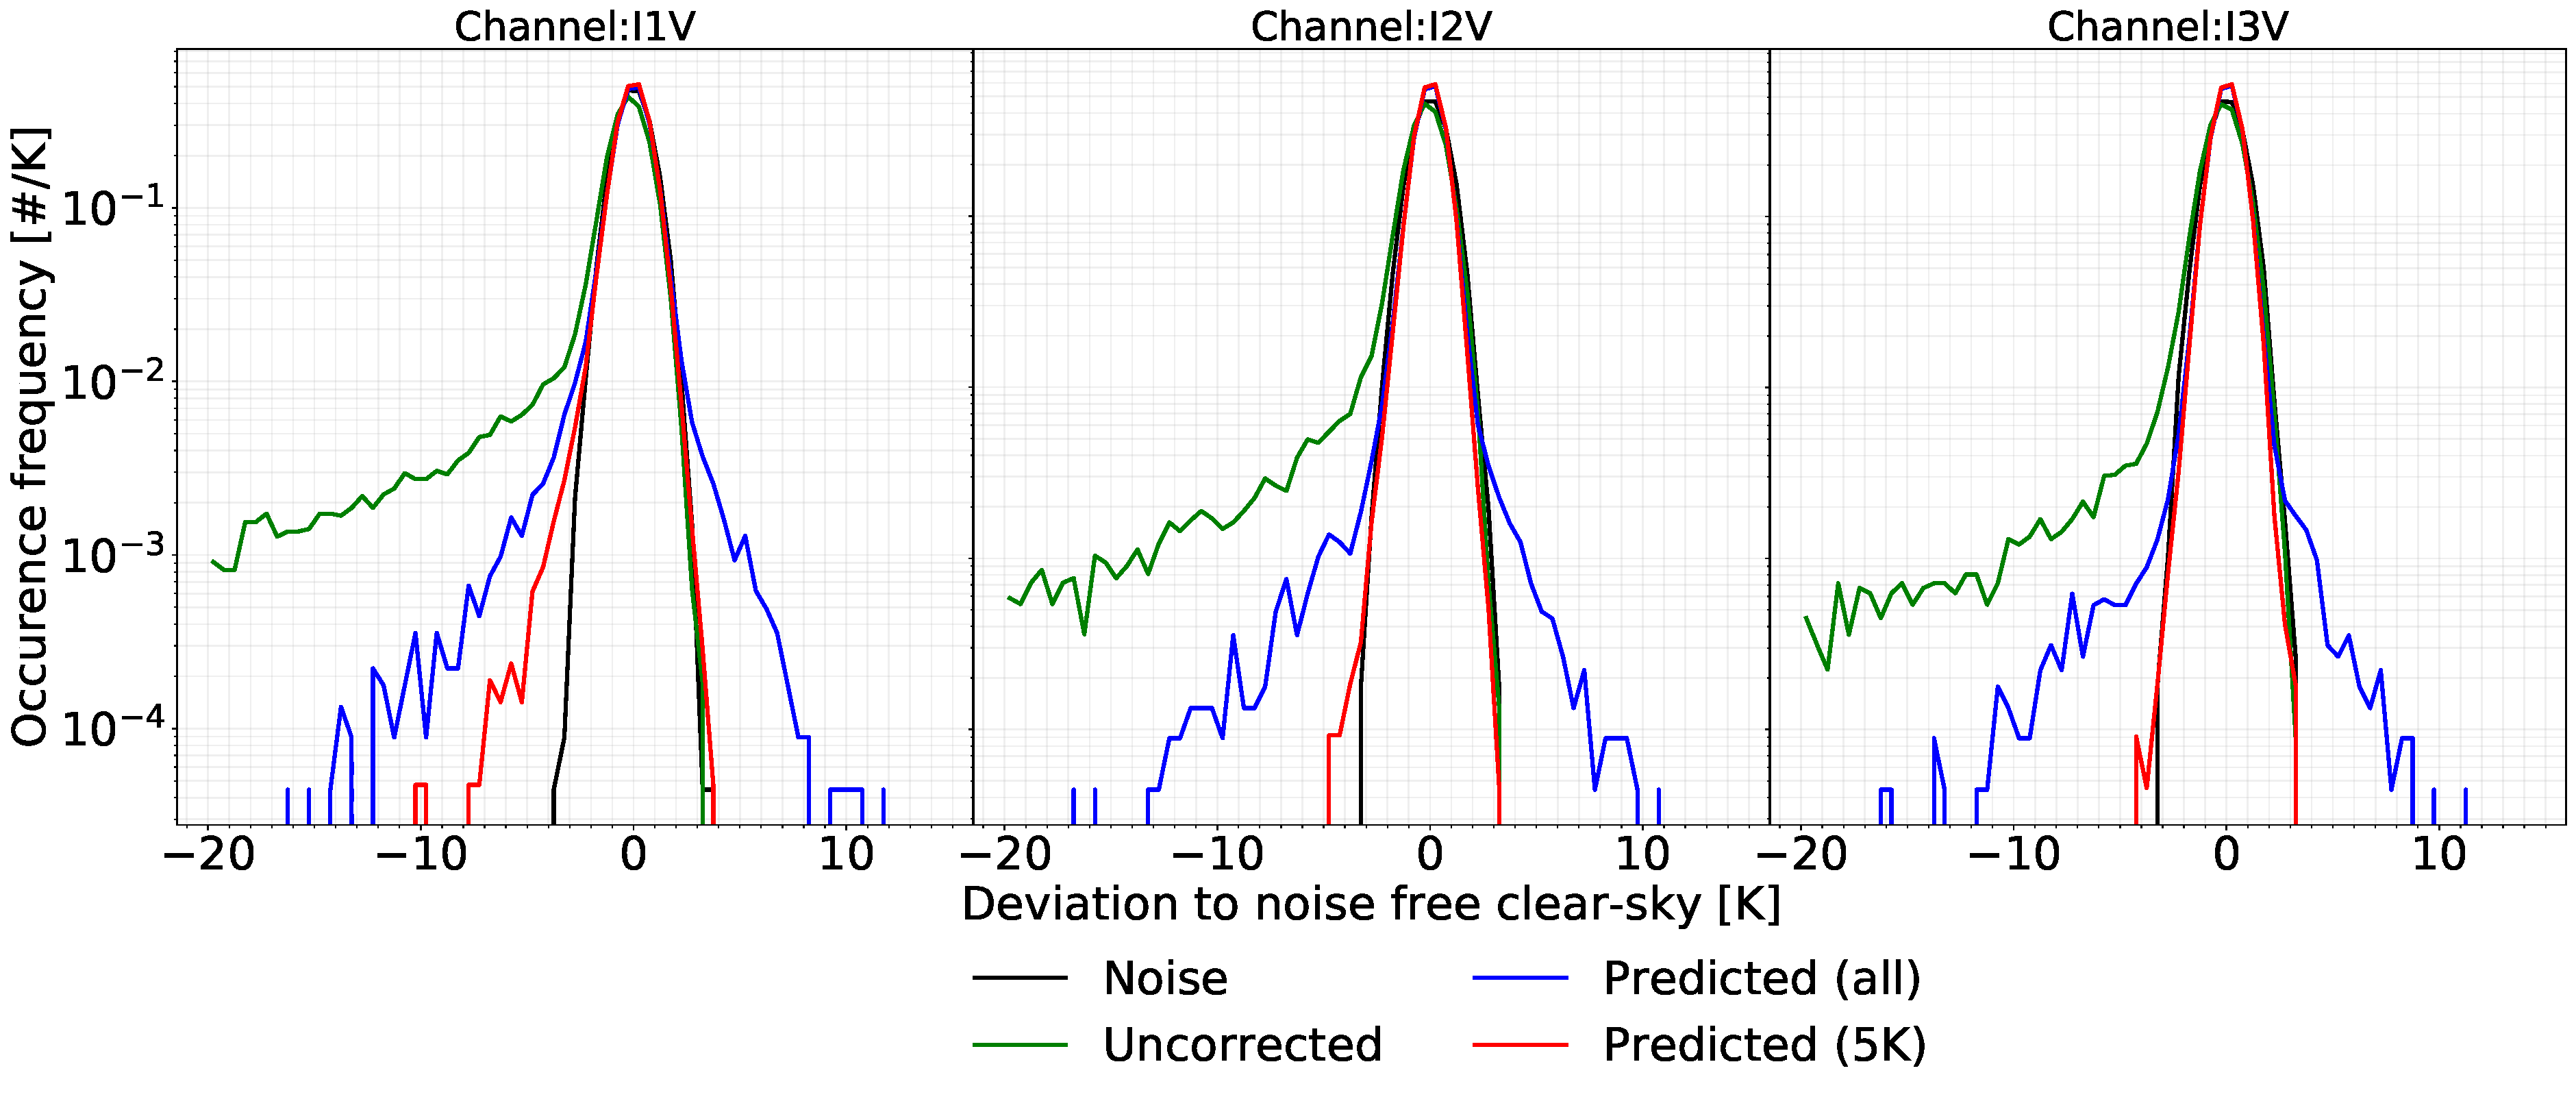
\includegraphics[width=\textwidth]{Figures/error_distribution_QRNN-single.pdf} 
	\caption{Error distributions for deviations predicted data to NFCS simulations. The results are from QRNN-ici and channels I1V, I2V and I3V. Noise for each channel is also plotted for reference. The label ``Uncorrected'' represents the measurement data, ``Predicted(All)'' denotes the entire prediction dataset, while ``Predicted(5\,K)'' refers to the predicted dataset but where cases with cloud correction greater than 5\,K are excluded.}
	\label{fig:error_distributions}	
\end{figure*}
\begin{table*}[t]
	\caption{ Error statistics for deviations predicted data to NFCS simulations. 
		The values for Bias, mean absolute error(MAE), standard deviation(STD), and measure of skewness(Skewness) are shown. Results are for channels I1V, I2V and I3V. The number in parentheses is the percentage of cases removed by filtering. The label ``Predicted(All)'' refers to the complete predicted dataset, while ``Predicted (5\,K)'' denotes the prediction dataset but where cases with cloud correction greater than 5\,K are excluded.}
	\label{tab:error_statistics_ici}
	%	\tabcolsep=0.11cm
	\begin{tabular}{llrr|rr}
		\tophline
		&&\multicolumn{2}{c|}{Simulations}& \multicolumn{2}{c}{QRNN-single} \\
		\cline{3-6}
		%		\hline
		&&   Clear-sky &   All-sky &  \multicolumn{2}{c}{Predicted}  \\
		&&			   &			&	(5\,K) & (All) \\
		\middlehline
		%		\multicolumn{7}{c}{Channel - I1V}\\
		
		I1V&  bias     &  0.00 & -1.87 & -0.02 & -0.00  \\
		&mae      &  0.64 &  2.32 &  0.70 &  0.60   \\
		&std      &  0.80 &  8.84 &  1.06 &  0.79   \\
		&skewness & -0.01 & -8.10 & -1.51 & -0.64  \\
		\middlehline
		I2V & bias     & 0.00 &  -1.04 &  0.00 &  0.01  \\
		&mae      & 0.64 &   1.53 &  0.57 &  0.51 \\
		&std      & 0.80 &   5.95 &  0.86 &  0.65 \\
		&skewness & 0.00 & -10.79 & -1.85 & -0.22  \\
		\middlehline	
		I3V & bias     & 0.01 &  -0.63 &  0.02 &  0.02  \\
		&mae      & 0.64 &   1.15 &  0.54 &  0.50  \\
		&std      & 0.80 &   4.27 &  0.80 &  0.63  \\
		&skewness & 0.01 & -13.37 & -1.51 & -0.13  \\
		\bottomhline
	\end{tabular}
	\belowtable{} % Table Footnotes
\end{table*}

Fig.~\ref{fig:PDF_predictions} shows the distribution of point estimates given by QRNN. For all three channels, an excellent agreement between the predictions and simulations is observed. This indicates that QRNN is successful in predicting NFCS values for majority of the cases. At lower brightness temperatures, the frequency of predictions is slightly smaller than simulations. This could be due to few QRNN predictions ending up with partially corrected cloud impact. 

The QRNN prediction accuracy is estimated by computing the deviation of the best estimate to its corresponding NFCS simulation(Fig.~\ref{fig:error_distributions}). The predicted values have symmetric error distributions albeit with a large spread. The large spread on the left is due to cases which end up with incomplete cloud correction, while the spread on the right is from cases where the predicted values are warmer than the simulations. For all three channels, quite similar behaviour is observed, though I1V has the most cases with residual cloud impact. If the predicted cases with correction more than 5\,K are rejected, the resulting error distributions fit the measurement noise, except for I1V, where cases with residual cloud impact introduces a negative bias. 

For a quantitative assessment of the errors, we calculated the error metrics described in Sect.~\ref{sec:validation} and the results are displayed in Table~\ref{tab:error_statistics_ici}. The average bias in I1V measurements is -1.87\,K, which reduces to -0.02\,K after cloud correction. The corresponding standard deviation is 1.06\,K in comparison to 8.84\,K in the measurements. The prediction accuracy of QRNN is further higher when filtering is made on the predictions. In this case, the residual bias zero, and the standard deviation is 0.79\,K, which is in fact of the order of measurement noise (0.80\,K). Similar results are seen for I2V, though a better performance is observed. In I2V, the measurement bias is -1.04\,K which reduces to zero after correction and the MAE improves by almost 60\%. Removing cases with correction greater than 5\,K from the predictions removes only 3.7\% of the data and reduces the absolute error further by 10\%. The standard deviation of the resulting dataset is only 0.65\,K as compared to 0.80\,K from noise. The reduction in the variability is also evident in the Fig~\ref{fig:error_distributions}, where the peak of distributions is sharper. In comparison to I1V and I2V, I3V has the lowest fraction of the measurements with significant cloud impact. In the predicted dataset, the bias is 0.02\,K and the MAE is 0.54\,K. Including correction along with filtering reduces the MAE further down to 0.50\,K and standard deviation to 0.63\,K.  

\subsubsection{AWS}

\begin{table*}[t]
	\caption{Same as Table~\ref{tab:error_statistics_ici}, but for AWS channels. }
	\label{tab:statistics_qrnn_aws}
	\begin{tabular}{llrr|rr}
		\tophline
		&&\multicolumn{2}{c|}{Simulations}& \multicolumn{2}{c}{QRNN-single} \\
		\cline{3-6}
		%		\hline
		&&   Clear-sky &   All-sky &   Predicted(All) & Predicted(5\,K) \\
		\middlehline
		AWS-32  &Bias     & 0.00 & -1.32 &  -0.03 & -0.02 \\
		&MAE      & 0.36 &  1.57 &   0.54 &  0.43 \\
		&STD      & 0.46 &  6.42 &   1.02 &  0.61 \\
		&skewness & 0.01 & -8.43 &  -0.07 & -1.98 \\
		\middlehline
		AWS-33	&Bias     & -0.01 & -0.98 &  0.02 &  0.01 \\
		&MAE      &  0.36 &  1.23 &  0.49 &  0.42 \\
		&STD      &  0.45 &  4.70 &  0.76 &  0.56 \\
		&skewness & -0.00 & -8.78 &  0.04 & -0.79 \\
		
		\middlehline
		AWS-34	&Bias     &  0.00 &  -0.68 &  0.02 &  0.01 \\
		&MAE      &  0.51 &   1.07 &  0.51 &  0.46 \\
		&STD      &  0.64 &   3.67 &  0.75 &  0.60 \\
		&skewness & -0.00 & -10.32 & -0.55 & -0.59 \\
		\middlehline
		AWS-35	&Bias     &  0.00 &  -0.43 &  0.01 &  0.00 \\
		&MAE      &  0.50 &   0.84 &  0.48 &  0.44 \\
		&STD      &  0.63 &   2.65 &  0.71 &  0.57 \\
		&skewness & -0.01 & -12.49 & -0.40 & -0.29 \\
		\middlehline
		AWS-36  &Bias     & 0.00 &  -0.28 &   0.03  &  0.03 \\
		&MAE      & 0.70 &   0.90 &   0.63  &  0.60 \\
		&STD      & 0.88 &   2.06 &   0.86  &  0.76 \\
		&skewness & 0.01 & -11.80 &  -0.35  & -0.20 \\
		\bottomhline				
	\end{tabular}
	\belowtable{} % Table Footnotes
\end{table*}
In an analogy between the results from ICI channels, we perform a similar error distribution analysis  and the results are displayed in Table~\ref{tab:statistics_qrnn_aws}. For channel AWS-32, the average bias and standard deviation in the uncorrected dataset is -1.32\,K and 6.42\,K respectively. However, after correction, the bias and standard deviation reduce to -0.03\,K and 1.02\,K. A decrease in the skewness of error distributions is evident, but a relatively high values after prediction indicate presence of cases with partially-corrected cloud impact. Filtering out cases with high cloud impact improves the statistics overall except for skewness, which increases.  For AWS-33, the predictions have slightly higher accuracy than AWS-32. The MAE in predictions is only 0.49\,K in comparison to 1.23\,K for the measurements. Low skewness and bias values indicate that the error distribution is quite symmetric. Similar results are also seen for AWS-35 and AWS-36. For both channels, the error distributions are relatively more symmetric than the other channels. Also, it is worth to noting that when cases with 5\,K cloud correction are removed, the spread of prediction errors is narrower than noise. 


\subsection{Prediction uncertainty}
\label{sec:prediction_uncertainty}
%f 
\begin{figure}[t]
	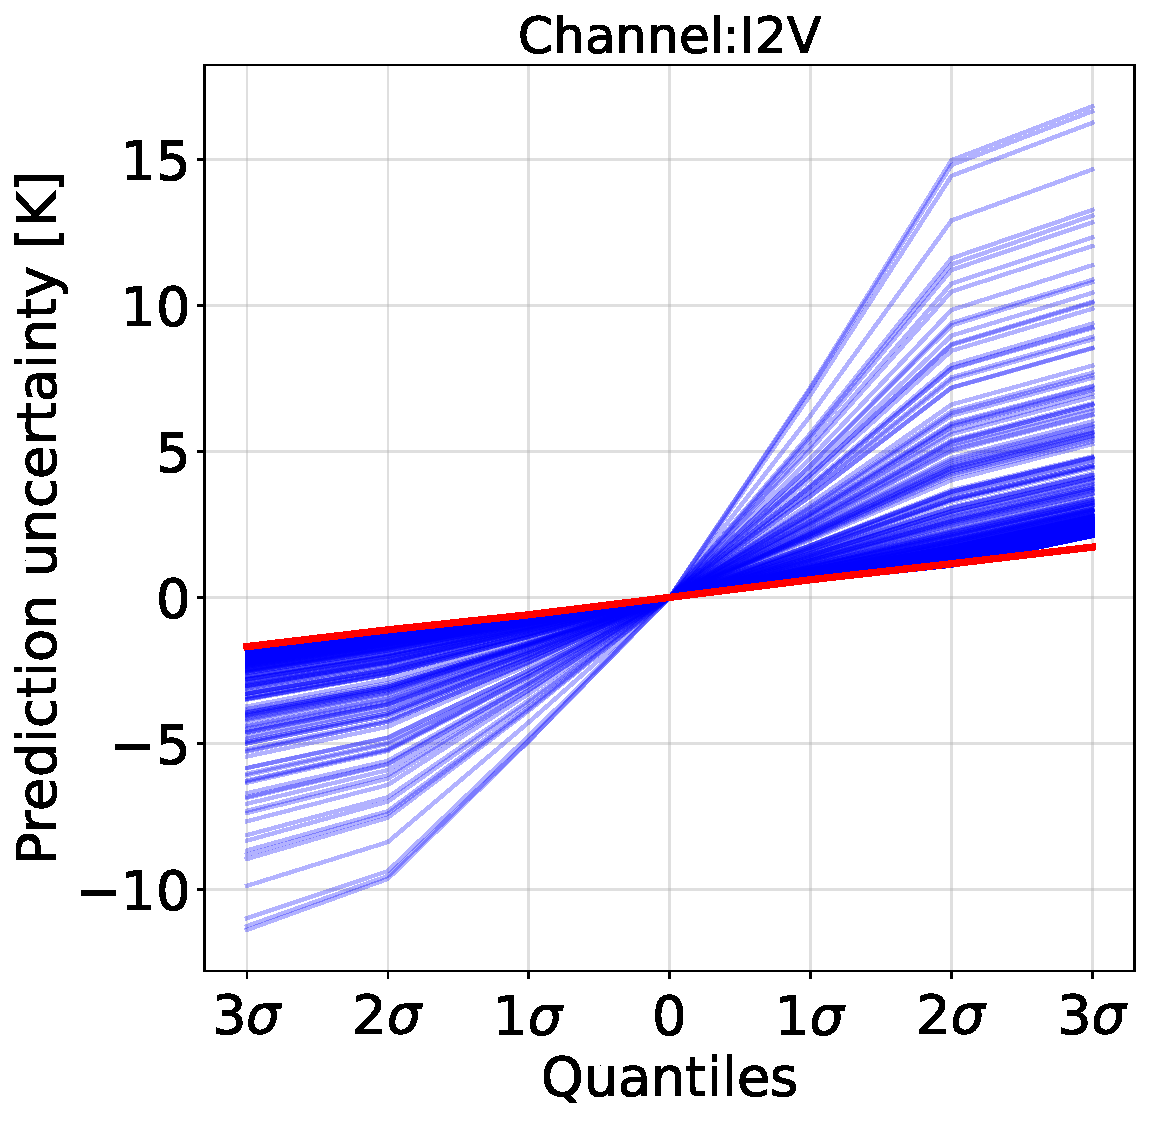
\includegraphics[width = 70mm]{Figures/prediction_uncertainty_I2V.pdf}	
	\caption{The prediction uncertainty for I2V (QRNN-single) with respect to quantiles for randomly selected 1500 cases. The quantiles have been plotted at equidistant points. The red line represents a hypothetical Gaussian distribution of $270\pm0.60$\,K, which is of the order of standard deviation for I2V predictions (see Table~\ref{tab:error_statistics_ici}).}
	\label{fig:prediction_uncertainty_I2V}	
\end{figure}
\begin{figure}[t]
	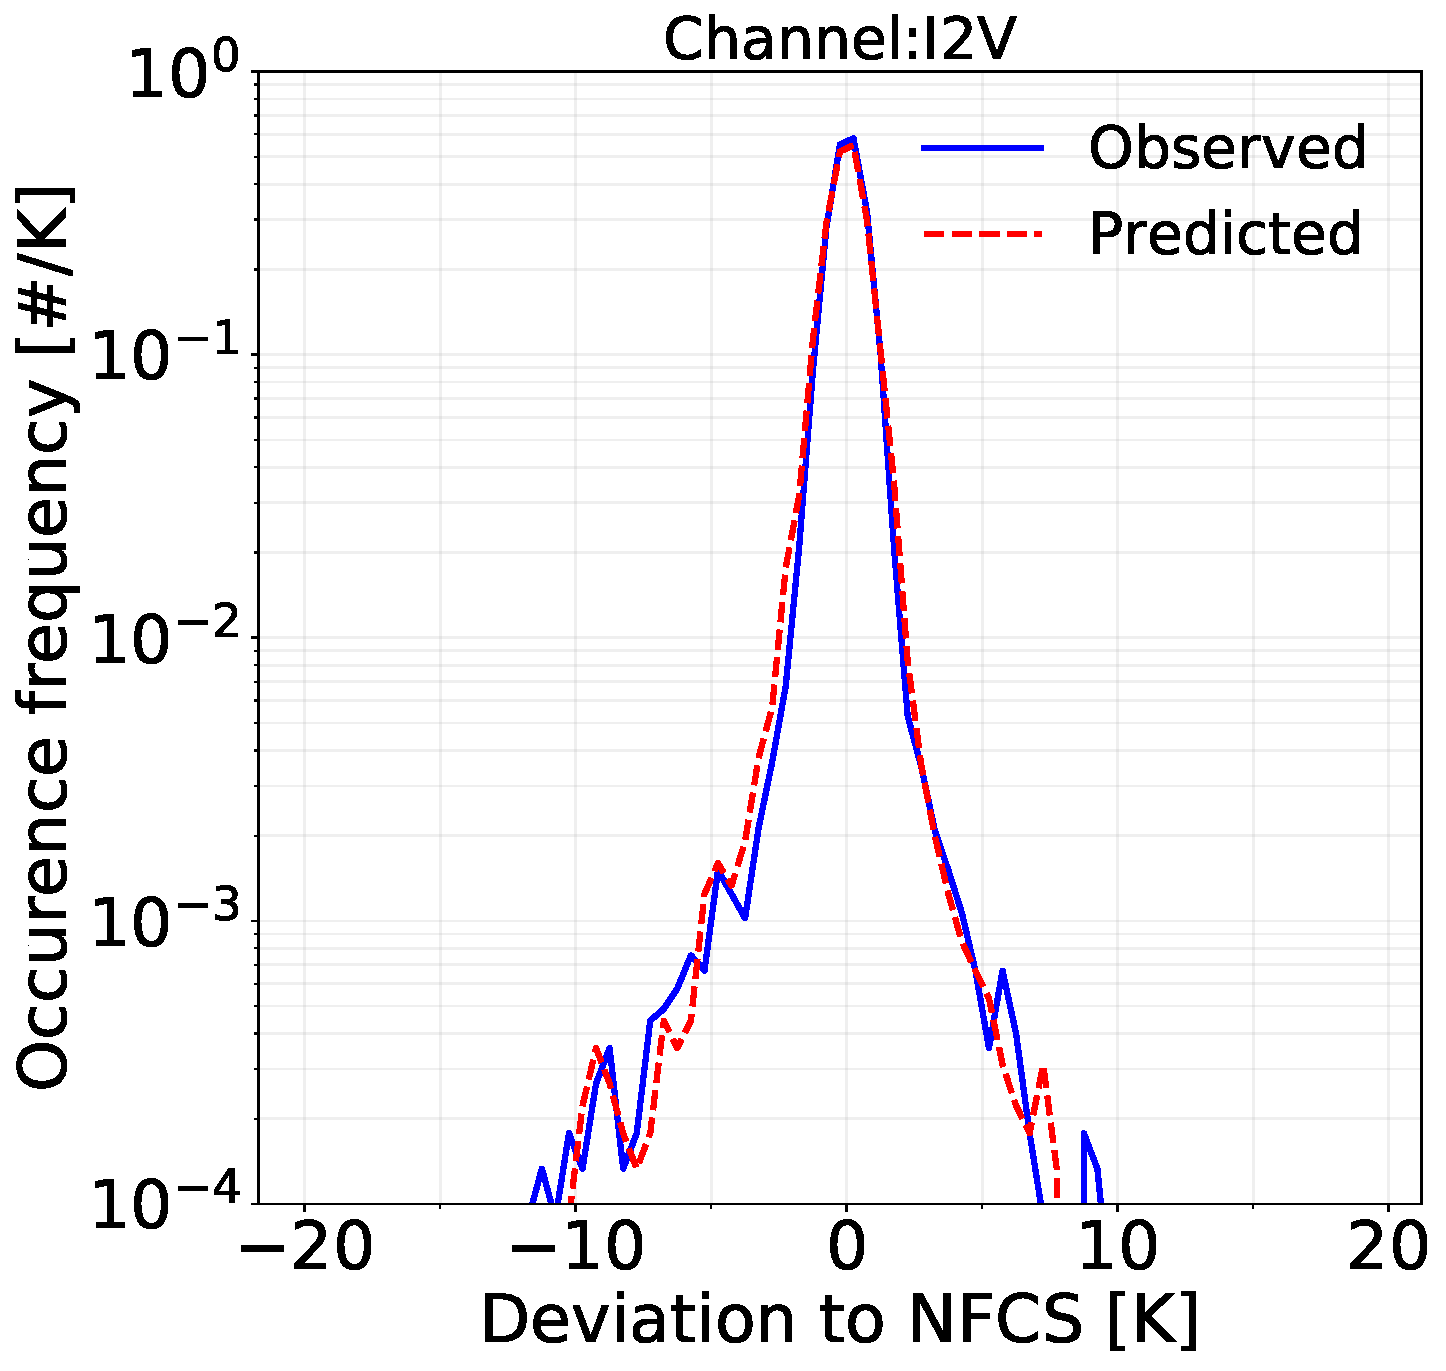
\includegraphics[width=70mm]{Figures/deviation_posterior_samples_I2V.pdf}	
	\caption{The distribution of predicted errors and observed errors for I2V as obtained from QRNN-single for the test dataset. The predicted errors are estimated as deviation of random samples from posteriori distribution to corresponding median values.}
	\label{fig:predicted_errors}	
\end{figure}
\begin{figure}[t]
	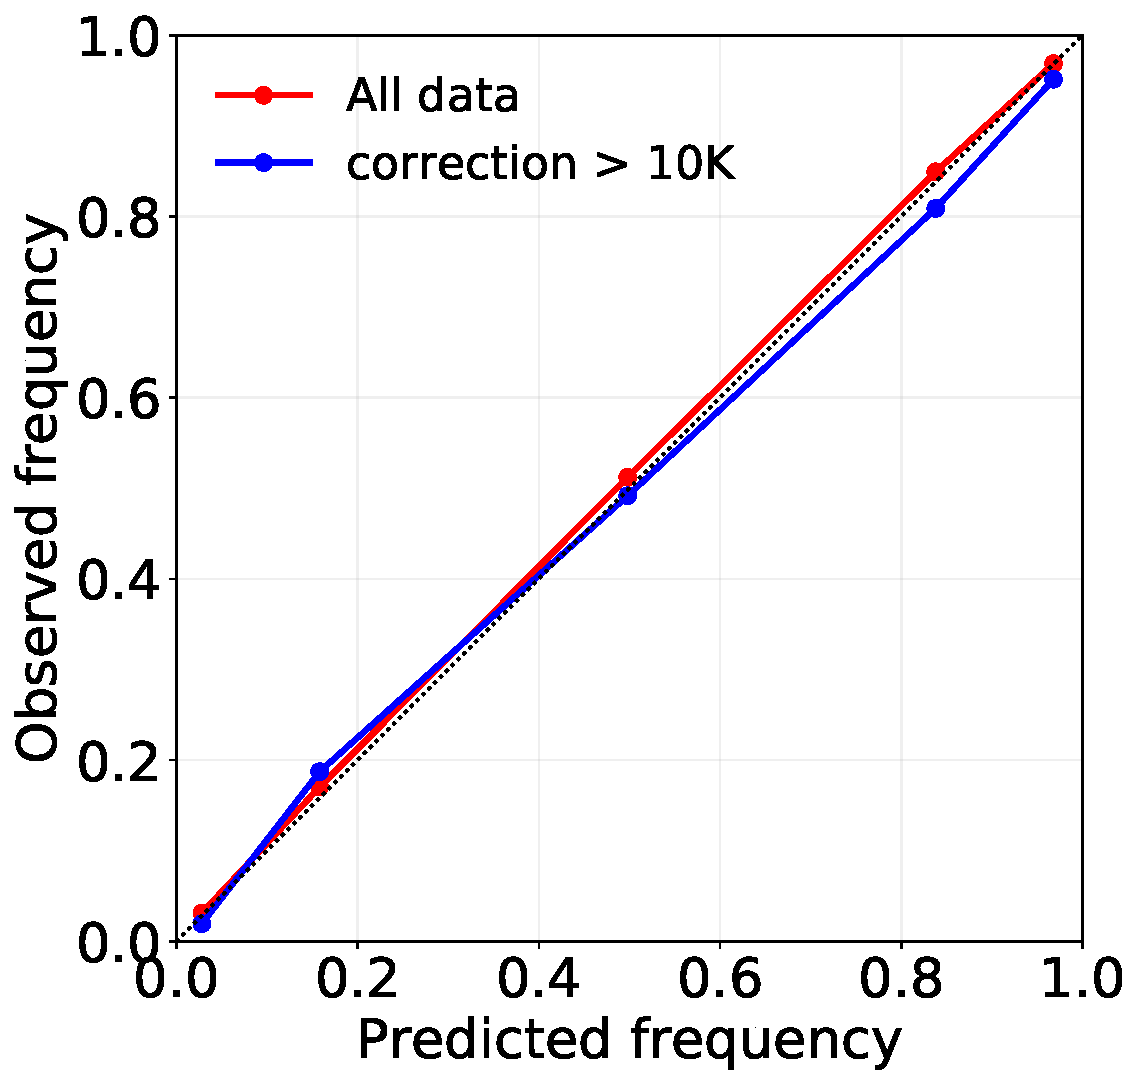
\includegraphics[height = 70mm]{Figures/calibration_QRNN_I2V.pdf}	
	\caption{Calibration of the prediction intervals obtained from QRNN-single for I2V. }
	\label{fig:calibration_I1V}	
\end{figure}
\begin{figure}[t]
	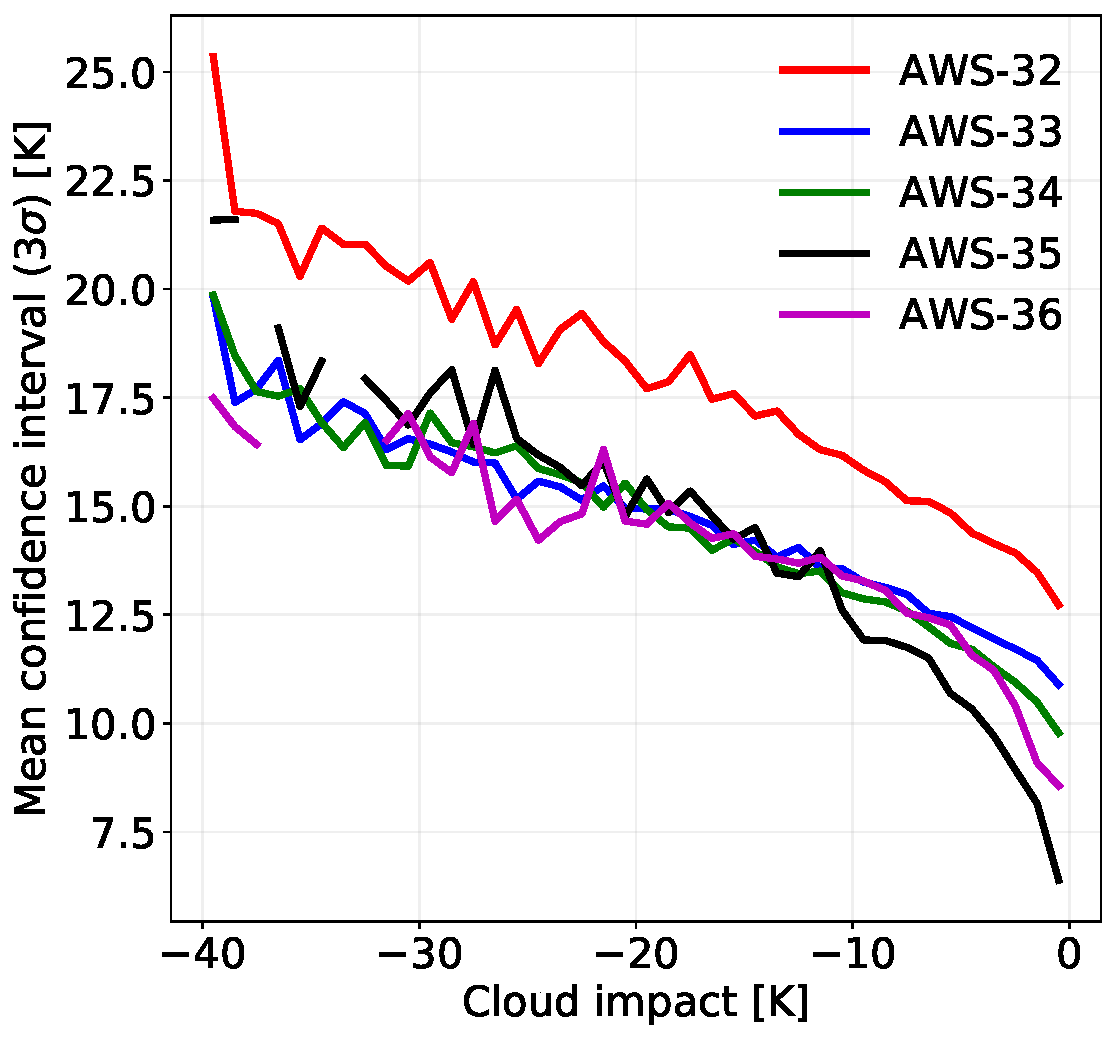
\includegraphics[width = 70mm]{Figures/cloud_impact_uncertainty_AWS.pdf}	
	\caption{The average confidence intervals (2$\sigma$) plotted against the magnitude of cloud impact for all AWS channels.}
	\label{fig:uncertainty_cloud_impact}	
\end{figure}
\begin{figure*}[t]
	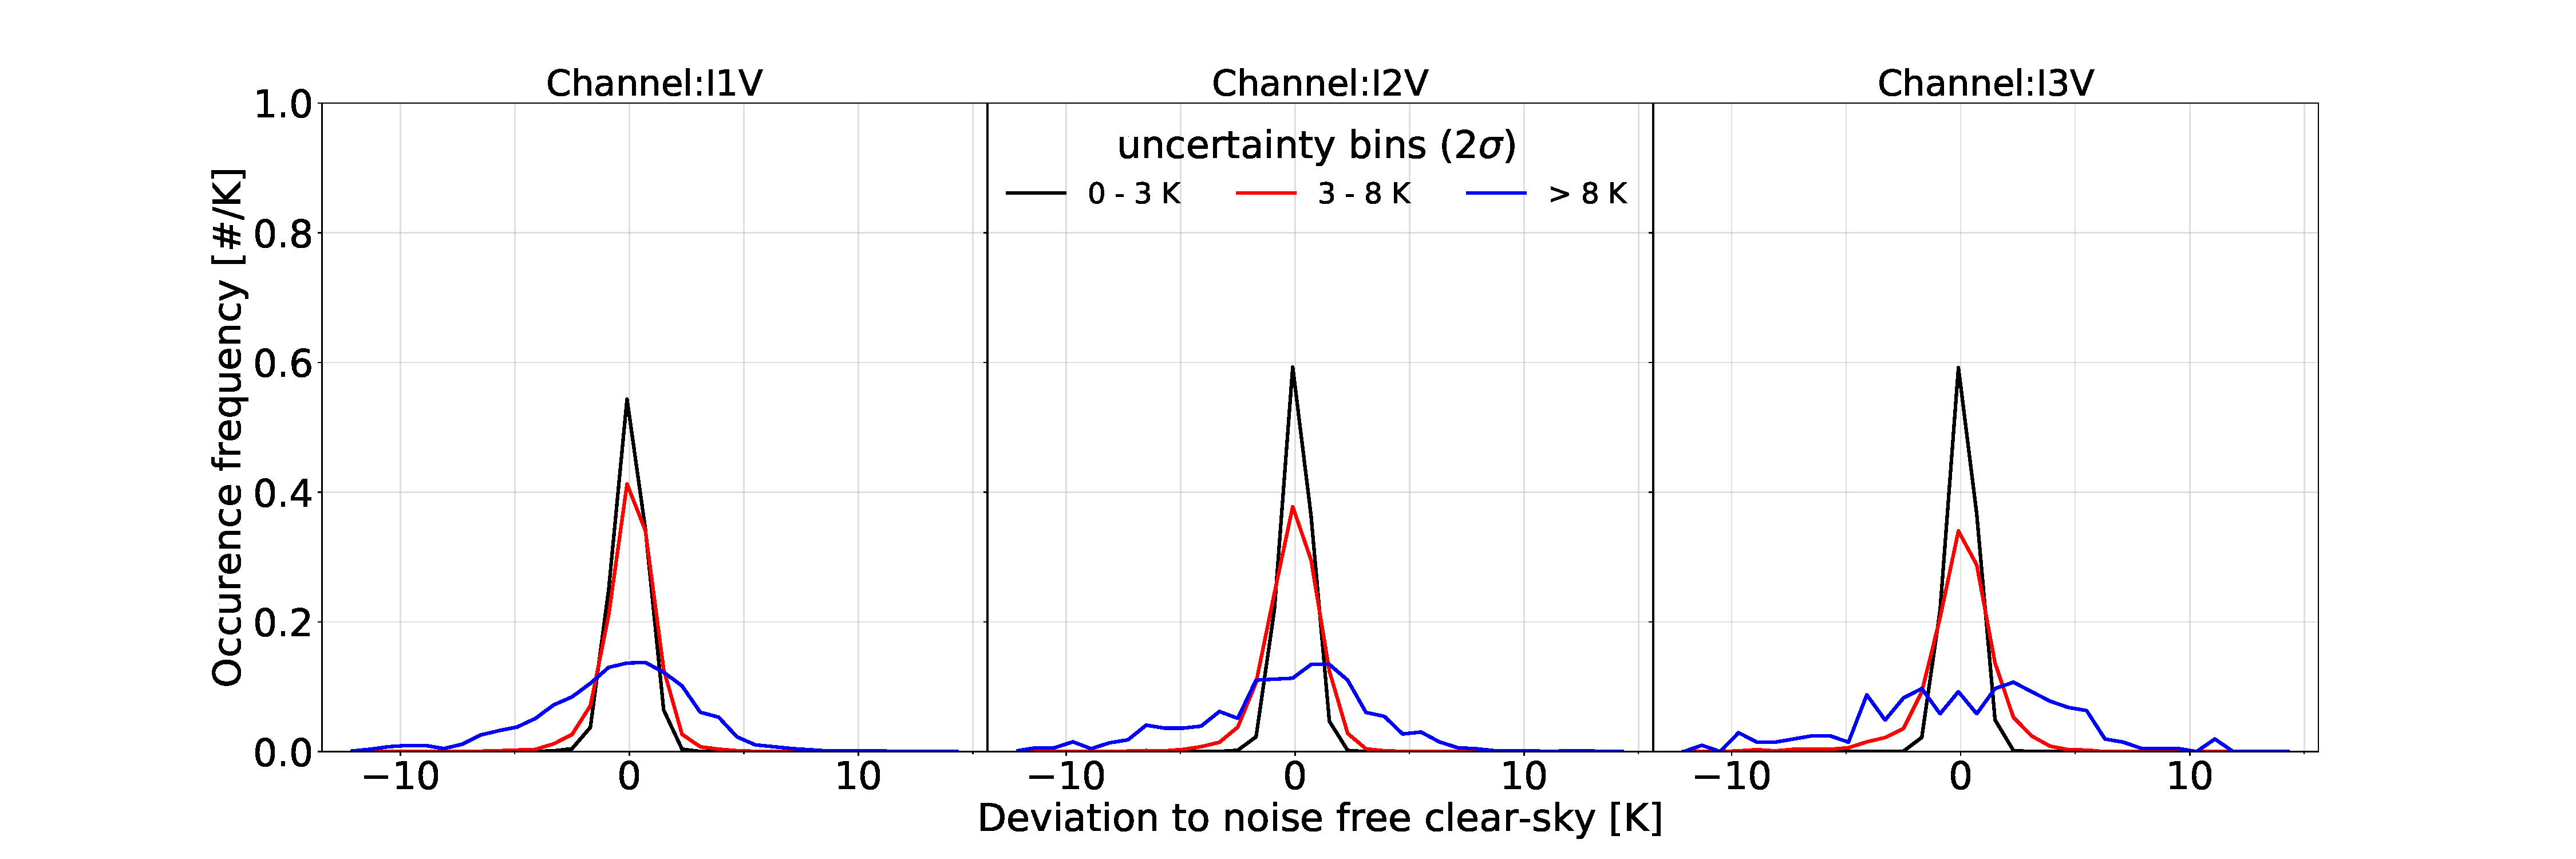
\includegraphics[width=\textwidth]{Figures/PDF_uncertainty_bins_QRNN-single.pdf}	
	\caption{Distribution of errors binned according to their uncertainty. Results are from QRNN-single for channels I1V, I2V and I3V.}
	\label{fig:error_distribution_uncertainty_bins}	
\end{figure*}
%f

Similar to evaluation of uncertainty estimates for MWHS-2(Sect.~\ref{sec:}), we analyse the spread of predicted quantiles, their calibration and distribution of predicted errors. 

Fig.~\ref{fig:prediction_uncertainty_I2V} shows the spread of prediction uncertainties over different quantiles for randomly chosen 1500 cases. The large spread in the predicted errors indicates that QRNN is successful in representing uncertainties for each case individually, rather than expressing them as a single measure for all cases. In the latter case, the uncertainty estimates would be concentrated along a narrow interval. Among the cases associated with low uncertainty, the distribution is quite symmetric along the median value. These cases are concentrated along a narrow interval and lie close to the red line representing a Gaussian spread. On the contrast, cases with high uncertainty are unequally spaced and have a larger spread over positive quantiles than negative quantiles. 

Fig.~\ref{fig:calibration_I1V} shows the calibration of the prediction intervals for I1V. The predictions for the complete test dataset are well calibrated and follow the y=x line. This shows that the training and test datasets come from the same a priori distribution. On the other hand, when only the cases with  cloud correction greater than 10\,K are considered, the predictions in all the intervals are poorly calibrated. In this case the calibration curve lies below the y=x line, indicating that the predicted intervals are too narrow, or the uncertainty is underestimated. 

Fig.~\ref{fig:predicted_errors} shows the comparison of observed errors (prediction accuracy) to predicted errors. The predicted and observed errors have good agreement for the peak of the distribution, but the predicted errors are spread out asymmetrically. QRNN is not able to represent the left wings of the distribution. This could also be a sampling issue, as the high errors we try to predict constitute a very small part of the complete dataset and we do not derive any sample from outside $\pm3\sigma$.   

With AWS, the behaviour of predicted uncertainties is observed to be similar as for ICI (not shown). However, the relation between the mean uncertainty estimate and cloud impact is displayed in Fig~\ref{fig:uncertainty_cloud_impact}. For all five channels, the predictions with small or relatively low cloud signal have a low uncertainty or in other words have high sharpness. As fraction of cloud impact increases, the predictions become increasingly uncertain. The most uncertain predictions are for the lowest peaking channel AWS-32, which incidentally is also most affected by  hydrometeor impact.  

To conclude the results, we assessed if the uncertainty estimates given by QRNN are representative of prediction accuracy. Fig.~\ref{fig:error_distribution_uncertainty_bins} shows the errors of best estimate binned by their corresponding uncertainty in $\pm2\sigma$  confidence interval. For all three channels, the spread of error distribution increases as the uncertainty about the accuracy of the trial increases. The cases with high certainty have a narrow and sharp distribution, and the errors are mostly less than $\pm$2.5\,K. With increase in the uncertainty, frequency of cases with high accuracy decreases and the distributions spread out symmetrically to higher errors. Poor predictions occur more frequently when uncertainty is high. Cases with accurate predictions yet high uncertainty are also present. In spite of individual variations in the error distributions for each channel, predictions and their corresponding uncertainties followed the same relationship. Similar results were also obtained with AWS(not shown). 


\section{Discussion}

\subsection{Cloud correction with existing sensors}
%
The results from MWHS-2 show that QRNN based cloud correction is partially successful in correcting the cloud impact with existing sensors. The methodology can correctly address the large negative depatures owing to cloud impact, but cases with low cloud impact end up with inadequate correction. The resulting error distributions are not completely symmetric but have a low bias and spread. Among several input channel combinations described for QRNN-single, the performance of combination 89+150\,GHz is observed to be optimal. The positive performance with 150\,GHz is not unexpected, as 150\,GHz is highly sensitive to ice hydrometeors and cloud water. But using 89\,GHz along with 150\,GHz gives a slightly better performance. The channel 89\,GHz is affected by surface emissivity and is relatively less sensitive to cloud water content, however its sensitivity to warm clouds in the lower troposphere could be important. We also investigate the impact of two temperature sounding channels (MWHS-2 channel 6 and 7). Both these channels provide complementary information to humidity channels in the lower troposphere. Including both these channels in the training process had no significant effect on the prediction accuracy. We obtain almost similar performance as with the combination 89+150\,GHz. 

Even though the cloud correction is partial, the performance is comparable or better to existing cloud filtering techniques like SI. SI is also a partial filter which identifies the contamination only due to precipitation and cloud ice. Note that SI is a one for all approach for all 183\,Ghz channels, thus is one observation is classfied as cloudy by SI, it is removed in all available humidity channels. This increases the probability of erroneously removing clear observations as cloudy. For high peaking channels of MWHS-2, both SI and QRNN give almost similar results, with however with almost 30\% rejection rate. On the other hand, for low peaking channels, the same rejection criteria gives less accurate results than QRNN. These channels have a stronger hydrometeor impact than channels 11 and 12. Clearly, a channel specific approach like QRNN is more appropriate and gives better performance.

The partial performance of QRNN is due to incomplete orthogonal information to 183\,GHz humidity channels.  The weighting functions of window channels 89 and 150\,GHz, and the two 118\,GHz channels peak in the lower troposphere. Among these four channels, 150\,GHz has the highest peaking function around 4\,Km \cite{chen2020mwhs}. These channels can only provide coverage to the humidity channels in lower and mid troposphere; nonetheless, the 183\,GHz channels are sensitive to hydrometeor content beyond 2\,Km. Due to missing complementary information from other channels in the upper troposphere, QRNN fails to train to predict these cases accurately. Additional information from other channels is necessary to help QRNN train better. Among the other available channels, the overlapping weighting functions of 183\,GHz can provide additional information to train QRNN. Though these channels help in improving the training, the non-orthogonal information introduces highly correlated observational errors. This is undesirable in data assimilation for NWP, but in future if the operational centres progress with approaches dealing correlated observation errors, using the configuration QRNN-all for cloud correction could be beneficial.

The biggest advantage of using QRNN is estimation of case-specific uncertainties. The predictions over chosen quantiles quantify the underlying uncertainty. The calibration plot and distribution of predicted errors show that  QRNN predictions are able to represent the a priori distribution.  However we also observe that cases with high errors are poorly calibrated. The poor calibration predictions associated with low accuracy is a consequence of different underlying a priori distribution. Predictions with high error originate from cases with high cloud impact. Such cases have a significantly distinct a priori distribtion as compared to clear cases, which dominate the training dataset, and influence the a priori information. Additional information in form of more observational data or additional training inputs is required to improve QRNN prediction accuracy for such cases. However such cases are rare and can be filtered out with simple threshold as showing earlier.
From data assimilation perspective, information on case-specific uncertainties is extremely useful. It allows for an effective selection of weights, thus significantly improving/deteriorating the impact of measurements. 


\subsection{Cloud correction with sub-mm frequencies }
%
In the ICI observations examined here, the results show that using sub-mm channels can successfully predict the NFCS values with very high accuracy for I2V, and I3V. The predicted values without any filter have an excellent match with the true values, and the departures are symmetrically distributed around zero mean. Few cases with high cloud impact do affect the accuracy and introduce a small negative bias, but such cases are easily filtered out with a simple correction threshold filter. For example, it is shown that filtering out cases with correction greater than 5\,K, results in variabilities of the order of noise with minimal reduction in data (2-4\%). For channel I1V, a slightly lower accuracy is observed due to relatively higher number of cases with residual cloud impact. The accuracy is improved by activating the correction filter, but some effect of residual cloud impact is apparent in the high negative skewness. Interestingly, reducing the correction threshold further has no significant effect on flagging these residual cases; in fact only the clear-sky cases are removed. This indicates that for I1V, QRNN is unsuccessful in correcting these cases completely. Compared to other two higher peaking channels, I1V is more sensitive to the effect of hydrometeors  and contamination from surface effects. The cases with surface contamination are also localized and seasonal. For QRNN to predict such cases accurately, QRNN should have access to complementary information from sub-mm channels. However, the weighting functions of sub-mm channels can provide only a partial coverage to the hydrometeor impact at I1V. A part of lower troposphere sensed by I1V has almost zero coverage from sub-mm channels. Though such cases are few, their lack of representation prevents QRNN from correctly learning to predict the clear-sky values accurately.

A similar pattern of results is seen for when only 325\,GHz channel is used to correct cloud impact in AWS. QRNN is successful in predicting NFCS values for all channels except for the lowest peaking channel AWS-32. For AWS-32, the resulting error distributions have significantly lower spread than the measurements, but are still negatively skewed. This indicates that a single sub-mm channel like 325\,GHz is also sufficient enough for cloud correction at 183\,GHz. This is an important result as smaller satellites are limited by their size to measure all sub-mm wavelengths.

With ICI and AWS, for some channels the variability of errors smaller than measurement noise is achieved. This is a consequence of predictions for cases which lack cloud impact. QRNN predictions are weighted mean of measurements between channels. For clear-sky conditions, multiple observations of same scene from different channels can cancel out the noise. This effect is observed to be stronger in ICI observations than AWS, due to more number of input channels while training in the former. It should be noted that with satellite measurements, the spread of error distributions smaller than noise could be difficult to achieve due to other underlying uncertainties not considered here. However, symmetric error distributions with low spread could still be extremely important from the context of data assimilation. Most of the existing cloud filtering schemes eg. \citet{buehler:aclou:07} and SI \cite{geer2015scatteringindex} work well only at removing cases with high cloud impact. As a consequence of the residual cloud impact, the error distributions are highly skewed. This is not the optimal solution but the best which can be achieved with present sensors. To use these observations correctly data assimilation schemes often inflate their asymmetric error distributions at the cost of artificially suppressing the observational impact.  

The analysis of QRNN predicted errors and calibration plots show that QRNN is successful in providing well calibrated probabilistic predictions of the posterior distributions except for few cases associated with high cloud impact. This is not unexpected as such cases form a small subset of the training set and their priori distribution is different from the entire dataset. 

\section{Conclusion and outlook}  %% \conclusions[modified heading if necessary]
%

In this study, a methodology based on quantile regression neural network (QRNN) is used for identifying and correcting the cloud contamination in operational humidity channels. QRNN is a neural network which trains on all-sky brightness temperatures from  channels containing orthogonal information to humidity channels, to estimate the noise free clear-sky (NFCS) radiances for humidity channels. The output is posterior distribution of the predictions over different quantiles. QRNN is a channel specific approach, or in other words, QRNN is trained separately for each channel, and the cloud correction for each is independent of other channels. 
 
The applicability of QRNN based correction to current sensors is demonstrated with MHWS-2 and it is shown that QRNN  is partially successful in removing the cloud impact. This is not optimal solution, but it is in agreement with what can be achieved with the present instruments. As compared to existing clear-filtering approaches, QRNN gives comparable or better performance and with minimal rejection of data. In context of present sensors, the accuracy of QRNN is affected by one single limitation, that is, the prediction of ``out of distribution'' cases. Predictions for such cases is always a challenging task for deep learning algorithms and shall always limit their performance. Improving the representation of such cases in the a priori distribution can help alleviate this problem to a certain extent. However, improving their priori distribution is not trivial when the no additional source of orthogonal information is present. 

Based on the promising results from MWHS-2, and with future scope, we extend the study to include data from sub-millimeter (sub-mm) channels. The results show that with  sub-mm channels, QRNN is able to correctly predict most of the cloudy cases and can provide high quality cloud corrected radiances. The predicted radiances have symmetric and narrow error distributions and for some channels the spread is smaller than the measurement noise. This makes it highly suitable for application to data assimilation systems.  The robustness of sub-mm channels in cloud correction is also demonstrated with use of only 325\,GHz for cloud correction. This is applicable to smaller satellite missions like AWS, where only one of the higher frequencies is available. The results indicate that utilisation of only 325\,GHz can also be beneficial when other channels are absent. In future when ICI would be available, the ICI sub-mm channels could also be used to cloud correct MWI humidity radiances. Although re-mapping to a common footprint would slighly compromise the data quality, the high accuracy achieved with ICI simulations suggests that the QRNN would work well even when actual measurements are available.


The biggest advantge of QRNN compared to other regression based approached is that its probabilistic nature. The QRNN predictions over chosen quantiles are a measure of the accuracy at different probability levels. In comparison to deterministic correction approaches, the corrected radiances along with uncertainty estimates. \todo{incomplete}  


The high quality cloud corrected radiances have great potential in DA systems. Most DA systems reject upto 80\% of the available observations due to cloud contamination. The loss is largest in mid-latitudes. Although, NWP systems are gradually moving towards assimilating all-sky radiances but the use of data is overly cautious. Misrepresentation of clouds can deteriorate the model outputs. To improve the representivity of clouds in the models, the observational errors are inflated as a function of the cloud amount. Most NWP centres use partial cloud identification approaches. On the contrary, cloud cleared microwave radiances offer forecast benefits without additional complexities. Another advantage of combining 183\,GHz and sub-mm for cloud correction is that NWP systems, which are not yet prepared for higher frequency channels, could still benefit from the data early on. 


%% The following commands are for the statements about the availability of data sets and/or software code corresponding to the manuscript.
%% It is strongly recommended to make use of these sections in case data sets and/or software code have been part of your research the article is based on.

\codeavailability{TEXT} %% use this section when having only software code available


\dataavailability{TEXT} %% use this section when having only data sets available


\codedataavailability{TEXT} %% use this section when having data sets and software code available


\sampleavailability{TEXT} %% use this section when having geoscientific samples available


\videosupplement{TEXT} %% use this section when having video supplements available


\appendix
\section{ARTS simulation setup}    %% Appendix A
\label{appendix:ARTS_setup}
%
**** Some parts copied directly from AWS report *****
Cloudsat profiles during August 2015 were randomly selected for forward simulations. The input data were restricted between $60^{\degree}$S to $60^{\degree}$N, and surface is below 500\,m. Both clear-sky and all-sky scenarios were simulated, and no differentiation was made between the observations over ocean/sea and land. 

The absorption model takes into account the effect from nitrogen
\citep{pwr:93}, oxygen \citep{pwr:93} and water vapour
\citep{ellison2007permittivity}. LWC is taken from ERA-Interim and is assumed
to be totally absorbing. In the mapping of CloudSat reflectivities to RWC and
IWC a total separation between liquid and ice phase is assumed. All scattering
hydrometeors at temperatures above 0$^\circ$C are assumed to be rain, and all
below 0$^\circ$C are assumed to be ice hydrometeors. For RWC the particle size
distribution of \citet{abel2012improved} is applied. The PSD of IWC follows the
basic formulation applied in DARDAR (\verb
http://www.icare.univ-lille1.fr/projects/dardar), using latest parameter
values (i.e.\ $\alpha$ and $\beta$) as given by \citet{cazenave2019evolution}.
This PSD can be considered as a ``two moment'' scheme, but is here applied in
a one moment manner by setting $N_0^*$ (as a function of temperature)
following Table~5 of \citet{delanoe2014normalized}, and letting the radar
reflectivity set the remaining moment. Single scattering data are taken from
\citet{eriksson:agene:18}. For ice hydrometeors, three habits are applied:
Perpendicular 3-bullet rosette, Large plate aggregate and Large column
aggregate. In the last two cases, the aggregates are complemented with single
crystal data to also cover smaller sizes. These data describe particles
assumed to have a totally random orientation. To apply oriented particles is
much more computationally costly and could not be accommodated inside the
study. The land emissivity was taken from TELSEM \citep{aires2011tool} and the
Ocean/water from TESSEM \citep{prigent2017sea}. For each atmopsheric case,
both ''clear-sky'' and ``all-sky'' calculations were performed. In the former,
all impact of all hydrometeors were set to zero, while in the latter, IWC and
RWC derived from CloudSat reflectivities and LWC from ERA-Interim were taken
into account. Both sets of calculations were made by ARTS's interface to the
RT4 solver \citep{evans1995microwavec}. To avoid a possible bias between
clear-sky and all-sky for insignificant hydrometeor contents, the same
``scattering solver'' was used for both calculations. The first two elements
of the Stokes vector were calculated.

\subsection{QRNN network structure}
\label{appendix:hyperparamter}
%
\begin{figure*}[t]
	\centering
	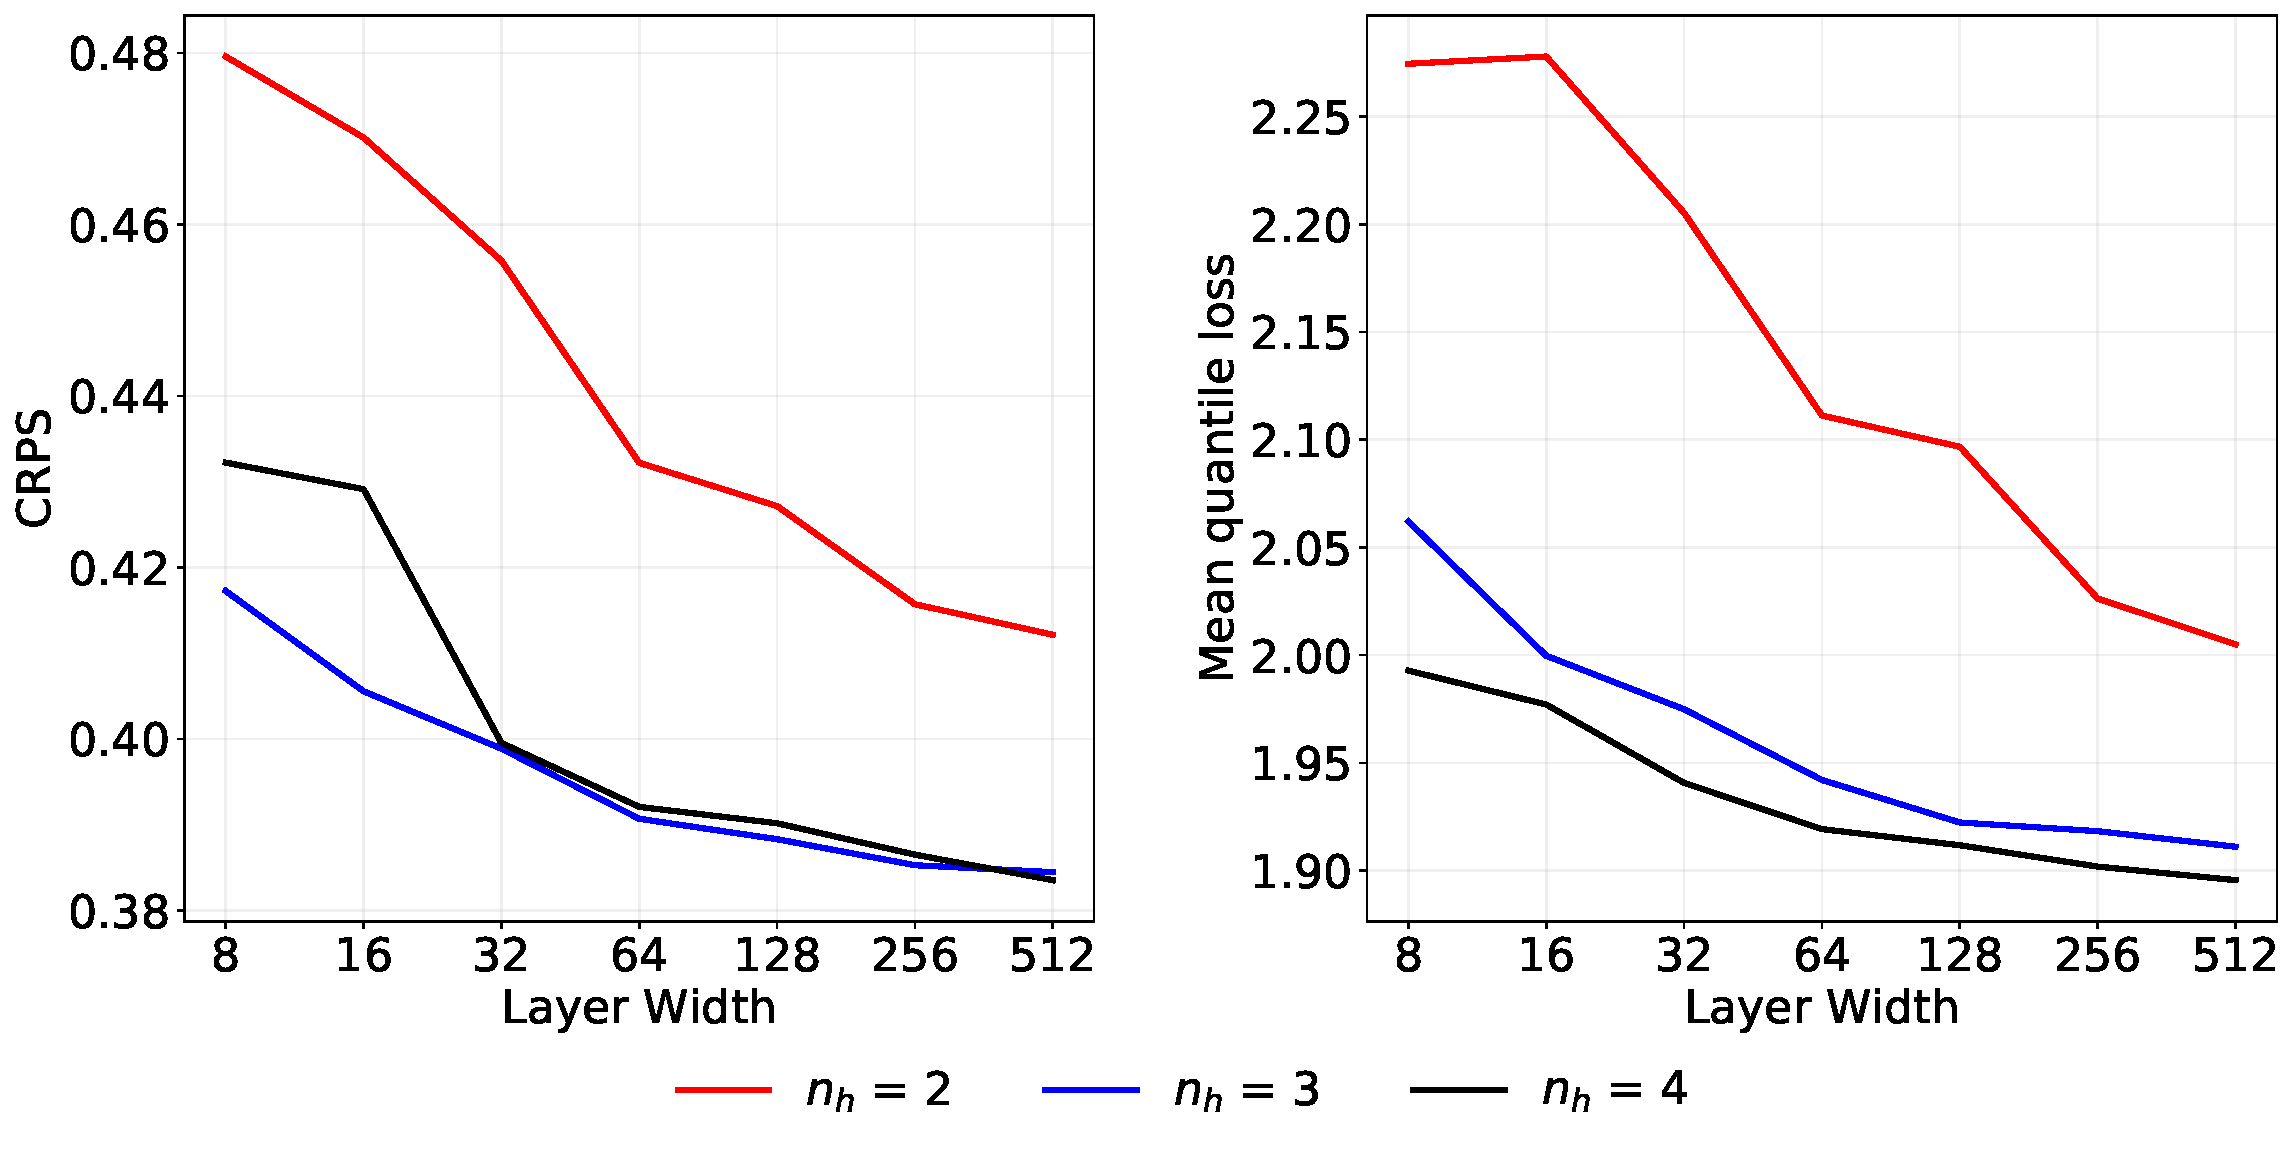
\includegraphics[height=60mm]{Figures/CRPS.pdf} 
	\caption{CRPS(left) and mean quantile loss(right) averaged over all predicted quantiles for different combinations of layer width and hidden layers ($n_h$). The results are from QRNN-single applied to I2V.}
	\label{fig:grid_search}	
\end{figure*}
A high performing QRNN model also requires tuning of multiple hyper-parameters. These parameters determine the structure and the training set-up of the neural network. Several of these hyper-parameters are non-learnable, and must be defined before beginning of every training. Grid search is one of the most often employed techniques for hyper-parameter tuning. In grid search, different combinations of hyper-parameters are selected and for each, the model performance is evaluated. The model architecture with the best performance is selected. For the structural parameters, usually a grid search over the number of neurons (width) and hidden layers (depth) is performed. The model is trained for multiple values of layer widths and hidden layers, and the best configuration is selected by evaluating the predictions over validation dataset. Similarly, the training process is optimized by performing a grid search different training parameters such as : batch size, learning rate, number of epochs etc. We use quantile loss and CRPS for evaluation of the model performance.

In this study, we investigated the performance of QRNN only to certain hyper-parameters like number of neurons, hidden layers, learning rate, convergence epochs and batch size. The optimization of other hyper-parameters was not performed and were chosen empirically. Firstly, we performed a grid search to define the structure of the neural network. We evaluated the performance for three sizes of hiddden layers($n_h$ = 2, 3, 4), and layer widths of sizes in the set [8, 16, 32, 64, 128, 256, 512]. The mean quantile loss and CRPS over all predicted quantiles was computed for each configuration (Fig.~\ref{fig:grid_search}). Increasing the complexity of the network by increasing the layer width and depth has a positive impact on performance. However for four hidden layers, increasing the number of neurons beyond 128 has no significant impact on the performance. On basis of these results, a neural network with four hidden layers and 128 neurons in each layer is selected. For optimising the training parameters, a customised  learning rate scheduler was implemented. The initial learning rate was reset after a certain number of epochs.  We started the training process with a initial learning rate of 0.1, and decreased it by a factor of 10 after 100 epochs. The best neural network performance was obtained when the network was trained three times. Each time with a new initial learning rate. For each training, if the validation loss remained unchanged till 6 training epochs, the learning rate was reduced by a factor of 2. 
In order to select the batch size, we simply compared the performance for two batch sizes: 128 and 256, and the former gave better results. Concerning number of epochs, we obtained best results when the network was trained longer. Choosing a lower value of epochs (e.g. 50), did not affect the accuracy of the median value, yet deteriorated the prediction uncertainty. We did not optimise the type of activation function and Rectified Linear Unit (ReLu) was used in all layers. 

Though these set of hyper-parameters were selected for QRNN-single applied to I2V, they worked well for both ICI and AWS QRNN experiments. However, for MWHS-2, an identical hyperparameter framework but three hidden layers gave best results.  

     %% Appendix A1, A2, etc.


\noappendix       %% use this to mark the end of the appendix section. Otherwise the figures might be numbered incorrectly (e.g. 10 instead of 1).

%% Regarding figures and tables in appendices, the following two options are possible depending on your general handling of figures and tables in the manuscript environment:

%% Option 1: If you sorted all figures and tables into the sections of the text, please also sort the appendix figures and appendix tables into the respective appendix sections.
%% They will be correctly named automatically.

%% Option 2: If you put all figures after the reference list, please insert appendix tables and figures after the normal tables and figures.
%% To rename them correctly to A1, A2, etc., please add the following commands in front of them:

\appendixfigures  %% needs to be added in front of appendix figures

\appendixtables   %% needs to be added in front of appendix tables

%% Please add \clearpage between each table and/or figure. Further guidelines on figures and tables can be found below.



\authorcontribution{TEXT} %% this section is mandatory

\competinginterests{TEXT} %% this section is mandatory even if you declare that no competing interests are present

\disclaimer{TEXT} %% optional section

\begin{acknowledgements}
TEXT
\end{acknowledgements}




%% REFERENCES


 \bibliographystyle{copernicus}
 \bibliography{references.bib}

\end{document}
